% -*- TeX-master: "multi" -*-

%%%%%%%%%%%%%%%%%%%%%%%%%%%%%%%%%%%%%%%
\section{Package syntax and semantics}
\label{def:Package_syntax_semantics}
%%%%%%%%%%%%%%%%%%%%%%%%%%%%%%%%%%%%%%%

This section contains a definition of the syntax and semantics of the Multi package for \SbmlLevelThreeCore.

% --------------------------------------------------------------------------
\subsection{Namespace URI and other declarations necessary for using this package}
\label{def:Namespace_URI}

The following is the namespace URI for this version of the Multi package for \SbmlLevelThreeCore:
\begin{center}
\uri{http://www.sbml.org/sbml/level3/version1/multi/version1}
\end{center}

In addition, SBML documents using a given package must indicate whether the package can be used to change the mathematical interpretation of a model. This is done using the attribute \attFont{required} on the \code{<sbml>} element in the SBML document. For the Multi package, the value of this attribute must be \val{true}.

The following fragment illustrates the beginning of a typical SBML model using \SbmlLevelThreeCore\ and this version of the Multi package:
\exampleFile{./examples/namespaces.xml}

% ------------------------
\subsection{Primitive data types}
\label{def:Primitive_data_types}

The Multi package uses a number of the primitive data types described in \sec{def:Namespace_URI} of the \SbmlLevelThreeCoreWC\ specification such as \SIdPT, \SIdRefPT, \stringPT, \booleanPT, \intPT\ and \positiveIntegerPT, and adds three additional primitive types described below.

\subsubsection{Type \BindingStatusPT}
\label{def:Primtype:BindingStatus}

The \BindingStatusPT\ primitive data type is used in the definition of the \OutwardBindingSite\ class.  \BindingStatusPT\ is derived from type \stringPT\ and its values are restricted to be one of the following possibilities: \val{bound}, \val{unbound}, and \val{either}.  Attributes of type \BindingStatusPT\ cannot take on any other values.  The meaning of these three values is discussed in the context of the \OutwardBindingSite\ class in \sec{def:OutwardBindingSite}.

\subsubsection{Type \RelationPT}
\label{def:Primtype:Relation}

The \RelationPT\ primitive data type is used in the definition of the \ListOfSpeciesFeatures\ class. \RelationPT\ is derived from type \stringPT\ and its values are restricted to be one of the following possibilities: \val{and}, \val{or}, and \val{not}. Attributes of type \RelationPT\ cannot take on any other values. The meaning of these three values is discussed in the context of the \ListOfSpeciesFeatures\ class in \sec{def:ListOfSpeciesFeatures}.

\subsubsection{Type \RepresentationTypePT}
\label{def:Primtype:RepresentationType}

The \RepresentationTypePT\ primitive data type is used in the extension of the \objFont{ci} element.\\ \RepresentationTypePT\ is derived from type \stringPT\ and its values are restricted to be one of the following possibilities: \val{sum} or \val{numericValue}. If present, attributes of type \RepresentationTypePT\ cannot take on any other values. The meaning of these values is discussed in the context of the  \objFont{ci} element in \sec{def:Reaction:Math:ci}.

% ------------------------
\subsection{The new and extended classes in the Multi Package}
\label{def:NewClasses}

The Multi package defines or extends the following object classes, \ExModel, \ListOfSpeciesTypes, \ExCompartment, \ListOfCompartmentReferences, \CompartmentReference, \SpeciesType, \ListOfSpeciesTypeInstances, \ListOfSpeciesFeatureTypes, \ListOfInSpeciesTypeBonds, \ListOfSpeciesTypeComponentIndexes, \SpeciesFeatureType, \ListOfPossibleSpeciesFeatureValues, \PossibleSpeciesFeatureValue, \SpeciesTypeInstance, \InSpeciesTypeBond, \SpeciesTypeComponentIndex, \ExSpecies, \ListOfOutwardBindingSites, \ListOfSpeciesFeatures, \OutwardBindingSite, \SpeciesFeature, \ListOfSpeciesFeatureValues, \SpeciesFeatureValue, \ExReaction, \ExSimpleSpeciesReference, \ExSpeciesReference, \ListOfSpeciesTypeComponentMapsInProduct, \SpeciesTypeComponentMapInProduct, \ListOfSpeciesFeatureChanges, and\\ \SpeciesFeatureChange.  

All the classes in the Multi package are directly or indirectly derived from \SBase, and \SBase provides the ability to attach \primtypeFont{SBO} terms as well as \primtypeFont{MIRIAM} annotations, the semantics of a given class in the Multi package can be made more precise by referencing to external controlled vocabularies and ontologies.

Like the classes in \SbmlLevelThreeCore, most new Multi classes have the attribute \idAtt\ (typically mandatory but not all, and of type \SIdPT), which serves as an identifier to provide a way to identify the class object. The identifier of a class object reference may or may not carry  mathematical interpretation or be used in mathematical formulas, depending on its class and the class object referencing it. The scope of \idAtt s is described in the section of ``Namespace scoping rules for identifiers''(\sec{def:namespaces_scoping_rules}). 

\clearpage

%------------------
\subsection{\Model}
\label{def:Model}

The Multi package extends the \Model class of \SbmlLevelThreeCore\ and adds an optional \ListOfSpeciesTypes child to \ExModel. \fig{fig:Model} provides the UML diagram for the extended \ExModel class.

\begin{figure}[htb]
  \begin{center}
    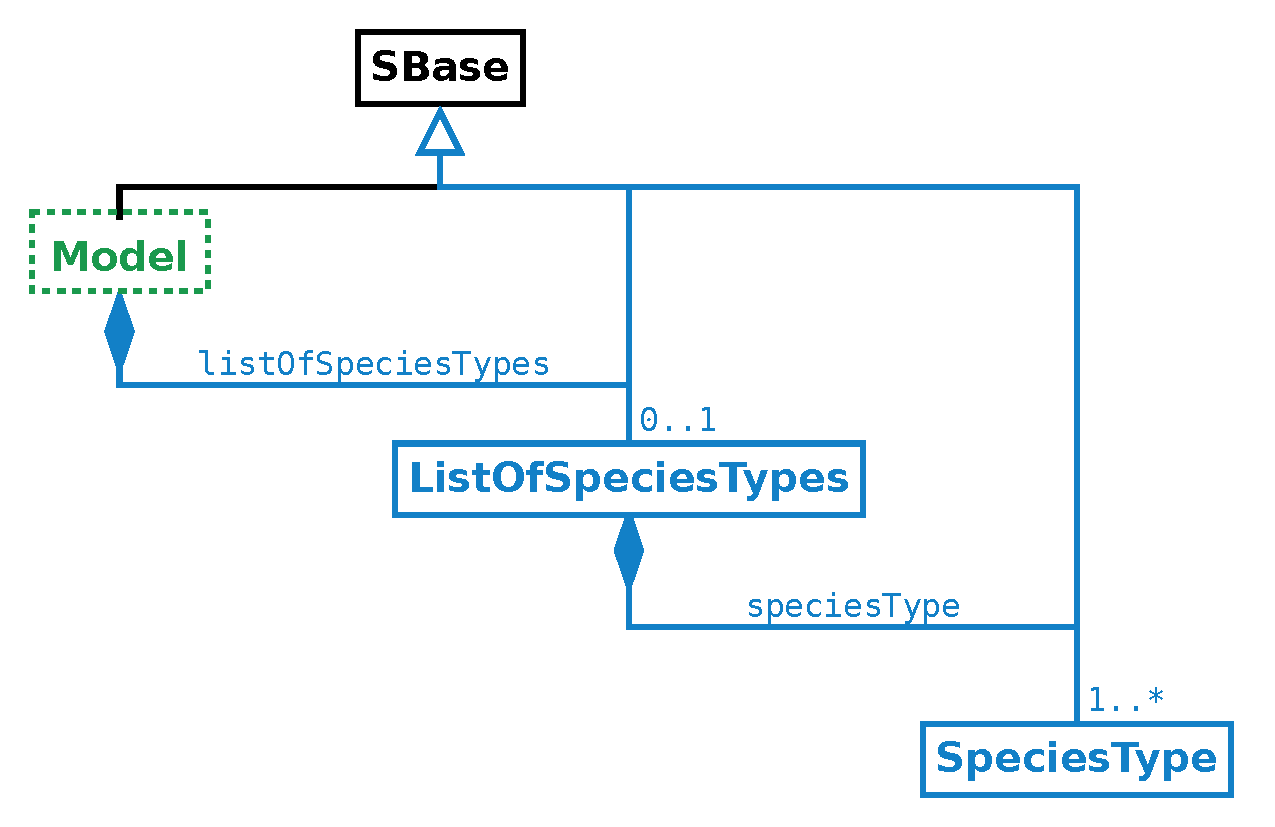
\includegraphics[scale=0.37]{./figs/multi_001_model.pdf}
    \caption{The extension of the \Model class.}
  \label{fig:Model}
  \end{center}
\end{figure}

%------------------
\subsubsection{\class{ListOfSpeciesTypes}}
\label{def:ListOfSpeciesTypes}

\class{ListOfSpeciesTypes} is defined in \fig{fig:Model}. If present, a \ListOfSpeciesTypes object must contain at least one \SpeciesType object.  Since \ListOfSpeciesTypes\ is derived from \class{SBase}, it inherits the \token{sboTerm} and \token{metaid} attributes, as well as the optional children \class{Notes} and \class{Annotation} objects. 

\clearpage

%-------------------------------
\subsection{Extended \class{Compartment}}
\label{def:Compartment}

A \Compartment object in \SbmlLevelThreeCore\ represents a bounded space in which \textit{species} are located. In the Multi package, \Compartment is extended. A Multi \compartment\ can be a \token{type} that multiple referencing \compartments\ can map to. A Multi \compartment\ can also be a composite \compartment\ or a container that includes other \compartments.

The extension of \class{Compartment} is defined in \fig{fig:Compartment_components}. The extended \Compartment class has a new required attribute \isTypeAtt, a new optional attribute \compartmentTypeAtt\ and an optional \ListOfCompartmentReferences child. The example at \sec{def:Example:CompartmentSpeciesTypeSpecies} illustrates the use of the extended \Compartment class.

\begin{figure}[htb]
  \begin{center}
    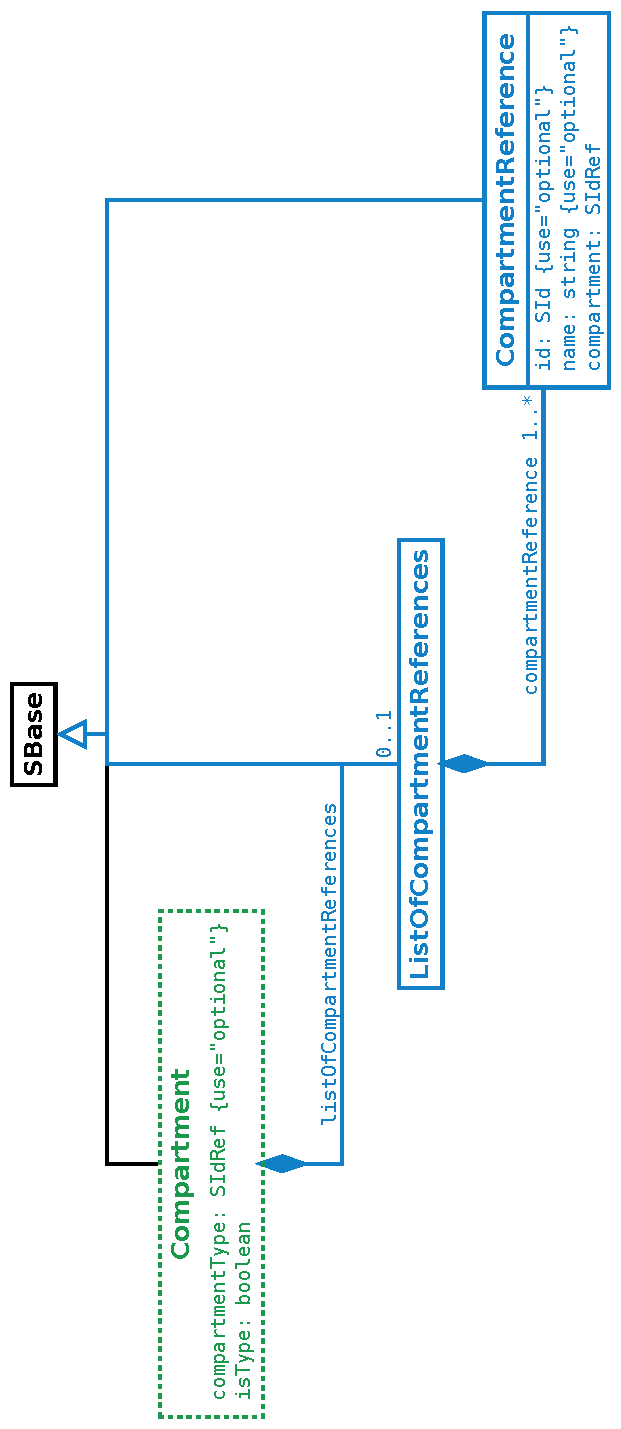
\includegraphics[angle=-90, scale=0.6]{./figs/multi_012_compartment.pdf}
    \caption{The definitions of \ExCompartment, \ListOfCompartmentReferences and \CompartmentReference}
  \label{fig:Compartment_components}
  \end{center}
\end{figure}

%--------------------------------------------------------
\subsubsection{The \isTypeAtt\ attribute}
\label{def:Compartment:isType}

The required attribute \isTypeAtt, of type \booleanPT, on the \class{Compartment} class serves to provide a way to indicate whether the \class{Compartment} object is a compartment type. 

A \class{Compartment} object is a compartment type if the value of its \isTypeAtt\ attribute is \val{true}. A \objFont{compartment type} is a template (in the sense of prototype) for all \class{Compartment} objects referencing it (via  \compartmentTypeAtt\ attributes). A \ExSpecies\ object directly referencing a compartment type is not a \fullydefinedspeciesWC. 

If the value of the \isTypeAtt\ attribute is \val{false},\label{def:Compartment:isType:false} the \class{Compartment} object is a \val{not-a-type} \textit{compartment} , and it is similar to a SBML core \compartment\ except it can reference a compartment type and can have a \ListOfCompartmentReferences child.

%-----------------------------------------------------------------
\subsubsection{The \compartmentTypeAtt\ attribute}
\label{def:Compartment:compartmentType}

The optional attribute \compartmentTypeAtt, of type \SIdRefPT, is used for a \val{not-a-type} \compartment\ to reference a compartment type. A \compartment\ with the \val{true} value of its \isTypeAtt\ attribute can not have the \compartmentTypeAtt\ attribute defined.

%-----------------------------------------------
\subsubsection{\class{ListOfCompartmentReferences}}
\label{def:ListOfCompartmentReferences}

\class{ListOfCompartmentReferences} is defined in \fig{fig:Compartment_components}, and must have one or more \CompartmentReference children.  Since \class{ListOfCompartmentReferences} is derived from \class{SBase}, it inherits the \token{sboTerm} and \token{metaid} attributes, as well as the optional children \class{Notes} and \class{Annotation} objects. 

\clearpage

%-------------------------------------------
\subsection{\class{CompartmentReference}}
\label{def:CompartmentReference}

\class{CompartmentReference} is defined in \fig{fig:Compartment_components}. It has two optional attributes \idAtt\ and \nameAtt, and a required attribute \compartmentAtt.  Since \class{CompartmentReference} is derived from \class{SBase}, it inherits the \token{sboTerm} and \token{metaid} attributes, as well as the optional children \class{Notes} and \class{Annotation} objects. 

%-----------------------------------------------------------------
\subsubsection{The \idAtt\ and \nameAtt\ attributes}
\label{def:CompartmentReference:idAndName}

The optional \idAtt\ attribute, of type \SIdPT, serves to provide a way to identify a \compartmentReference. \CompartmentReference also has an optional \nameAtt\ attribute, of type \stringPT. 

 If some or all \compartmentReferences\ within a \ListOfCompartmentReferences\ object reference the same \attFont{compart\-ment}, those \compartmentReferences\ are required to have their \idAtt\ attributes defined to distinguish different \compartmentReferences. 

%-----------------------------------------------------------------
\subsubsection{The \compartmentAtt\ attribute}
\label{def:CompartmentReference:compartment}

The required \compartmentAtt\ attribute, of type \SIdRefPT, serves to provide a way to reference a \ExCompartment\ object. 

%-----------------------------------------------
\subsection{The relationship of \class{Compartment}, \class{CompartmentReference} and \class{ListOfCompartmentReferences}}
\label{def:Relationships_CompartmentReferences}

In a \class{ListOfCompartmentReferences} object, every children \compartmentReferences\ must exclusively reference, directly or indirectly, \val{not-a-type} \compartment\ which can be of the same compartment type. See the extended \ExCompartment\ objects in the example in \sec{def:Example:CompartmentSpeciesTypeSpecies}.

All \compartments\ referenced by a \listOfCompartmentReferences\ must have the values of their \isTypeAtt\ attributes the same as that in the parent \compartment\ of the \listOfCompartmentReferences. For example, a compartment \val{A} with \isTypeAtt=\val{true} has a \listOfCompartmentReferences\ referencing two compartments \val{A1} and \val{A2}. Then, \val{A1} and \val{A2} must have \isTypeAtt=\val{true}. 

\clearpage

%-------------------------------------
\subsection{\class{SpeciesType}}
\label{def:SpeciesType}

\class{SpeciesType} is defined in \fig{fig:SpeciesType} and serves to provide backbone structures for \species. \class{SpeciesType} has  one required attribute, \idAtt, two optional attributes, \nameAtt\ and \compartmentAtt\ and four optional \class{ListOf\rule{0.15in}{0.5pt}} objects of \ListOfSpeciesFeatureTypes, \ListOfSpeciesTypeInstances, \ListOfInSpeciesTypeBonds\ and \ListOfSpeciesTypeComponentIndexes\ respectively.  Since \class{SpeciesType} is derived from \class{SBase}, it inherits the \token{sboTerm} and \token{metaid} attributes, as well as the optional children \class{Notes} and \class{Annotation} objects.  

The \ListOfSpeciesTypeInstances\ subobject provides a way to define multicomponents which are instances of other \class{SpeciesType} objects. 

The \ListOfSpeciesFeatureTypes\ subobject and its \SpeciesFeatureType\ children set up a framework for the referencing \species\ or the instances of \speciesTypes\ to be able to have multistates. The \ListOfSpeciesTypeComponentIndexes\ subobject provides a flexible way to reference any \component\ in a \speciesType. 

\begin{figure}[htb]
  \begin{center}
    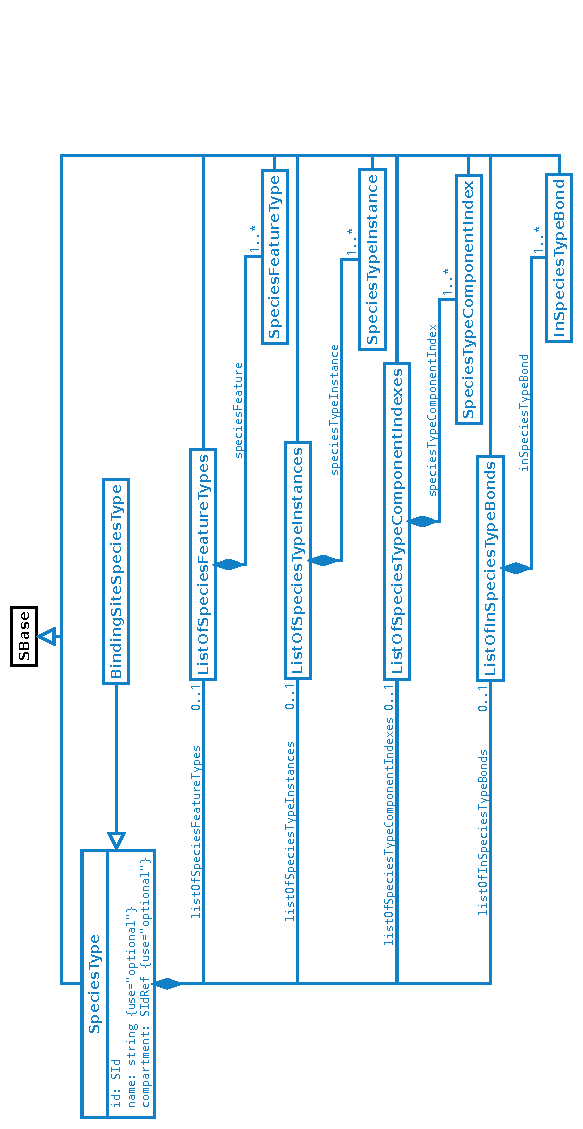
\includegraphics[angle=-90, scale=1]{./figs/multi_002_speciesType.pdf}
    \caption{The definition of the \SpeciesType class.}
  \label{fig:SpeciesType}
  \end{center}
\end{figure}

%-----------------------------------------------------------------------------------
\subsubsection{The \idAtt\ and \nameAtt\ attributes}
\label{def:SpeciesType:idAndName}

The required \idAtt\ attribute, of type \SIdPT, serves to provide a way to identify a \speciesType. \class{SpeciesType} also has an optional \nameAtt\ attribute, of type \stringPT. 
               
%---------------------------------------------------------------
\subsubsection{The \compartmentAtt\ attribute}
\label{def:SpeciesType:compartment}

\class{SpeciesType} has an optional attribute \compartmentAtt, of type \SIdRefPT, to be used to identify the \compartment\ where the \speciesType\ is located. The attribute value must be the identifier of an existing \compartment\ in the \model. If present, it must be consistent with the \compartmentAtt\ attributes of the referencing \species\ (see \sec{def:ExSpecies}) and the \compartmentReferenceAtt\ attributes of its instances (see \sec{def:SpeciesTypeInstance:compartmentReference}). The example in \sec{def:Example:CompartmentSpeciesTypeSpecies} illustrates how to keep the consistency of this attribute.

%--------------------------------------------
\subsubsection{\class{ListOfSpeciesFeatureTypes}}
\label{def:ListOfSpeciesFeatureTypes}

\class{ListOfSpeciesFeatureTypes} is defined in \fig{fig:SpeciesType}, and, if present, must have one or more \SpeciesFeatureType\ children.  Since \class{ListOfSpeciesFeatureTypes} is derived from \class{SBase}, it inherits the \token{sboTerm} and \token{metaid} attributes, as well as the optional children \class{Notes} and \class{Annotation} objects. 

%--------------------------------------------
\subsubsection{\class{ListOfSpeciesTypeInstances}}
\label{def:ListOfSpeciesTypeInstances}

\class{ListOfSpeciesTypeInstances} is defined in \fig{fig:SpeciesType}, and, if present,  must have one or more \SpeciesTypeInstance children.  Since \class{ListOfSpeciesTypeInstances} is derived from \class{SBase}, it inherits the \token{sboTerm} and \token{metaid} attributes, as well as the optional children \class{Notes} and \class{Annotation} objects. 

%--------------------------------------------
\subsubsection{\class{ListOfInSpeciesTypeBonds}}
\label{def:ListOfInSpeciesTypeBonds}

\class{ListOfInSpeciesTypeBonds} class is defined in \fig{fig:SpeciesType}, and, if present,  must have one or more \InSpeciesTypeBond children.  Since \class{ListOfInSpeciesTypeBonds} is derived from \class{SBase}, it inherits the \token{sboTerm} and \token{metaid} attributes, as well as the optional children \class{Notes} and \class{Annotation} objects. 

%--------------------------------------------------------
\subsubsection{\class{ListOfSpeciesTypeComponentIndexes}}
\label{def:ListOfSpeciesTypeComponentIndexes}

\class{ListOfSpeciesTypeComponentIndexes} is defined in \fig{fig:SpeciesType}, and, if present,  must have one or more \SpeciesTypeComponentIndex\ children.  Since \class{ListOfSpeciesTypeComponentIndexes} is derived from \class{SBase}, it inherits the \token{sboTerm} and \token{metaid} attributes, as well as the optional children \class{Notes} and \class{Annotation} objects. 

%--------------------------------------------------------

\subsubsection{\class{BindingSiteSpeciesType}}
\label{def:BindingSiteSpeciesType}

\class{BindingSiteSpeciesType} inherits the \SpeciesType\ class and is defined in \fig{fig:SpeciesType}. A \class{BindingSiteSpeciesType} object is a \objFont{binding site}, and therefore its instance can further define the \bindingStatusAtt\ attribute and can participate a binding internally and explicitly in an \InSpeciesTypeBond\ object, or externally and implicitly defined by an \OutwardBindingSite object. A \objFont{binding site} must be an atomic component which means that a \class{BindingSiteSpeciesType} object can not contain a \ListOfSpeciesTypeInstances\ subobject.


\noticeFont{Note: \notice \\
\label{def:OneToOneBinding}
In the Multi package, a \objFont{binding site} can participate one binding at a time. That means a \objFont{binding site} can not bind two partners at the same time. The binding relationship is one-to-one.
}

\clearpage

%-----------------------------------------
\subsection{\class{SpeciesFeatureType}}
\label{def:SpeciesFeatureType}

\class{SpeciesFeatureType} is defined in \fig{fig:SpeciesFeatureType}, and serves to provide frameworks or templates to define the referencing \SpeciesFeature objects. \class{SpeciesFeatureType} has two required attributes \idAtt\ and \occurAtt, an optional attribute \nameAtt,  and a required child \listOfPossibleSpeciesFeatureValues. The multiple \possibleSpeciesFeatureValues\ of the \ListOfPossibleSpeciesFeatureValues\ object permit constructing multistate \species\ via its \speciesFeatures\ under the \ListOfSpeciesFeatures object. Since \class{SpeciesFeatureType} is derived from \class{SBase}, it inherits the \token{sboTerm} and \token{metaid} attributes, as well as the optional children \class{Notes} and \class{Annotation} objects. 

\begin{figure}[htb]
  \begin{center}
    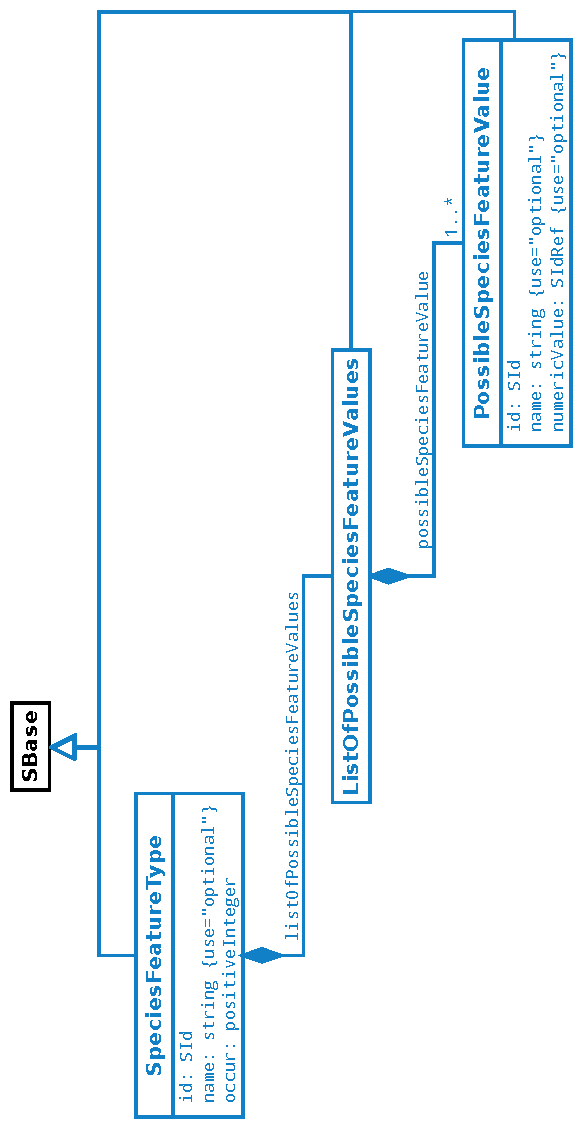
\includegraphics[angle=-90, scale=0.68]{./figs/multi_003_speciesFeatureType.pdf}
    \caption{The definitions of \SpeciesFeatureType, \ListOfPossibleSpeciesFeatureValues and \PossibleSpeciesFeatureValue classes. }
  \label{fig:SpeciesFeatureType}
  \end{center}
\end{figure}

%-----------------------------------------------------------------------------------
\subsubsection{The \idAtt\ and \nameAtt\ attributes}
\label{def:SpeciesFeatureType:idAndName}

The required \idAtt\ attribute, of type \SIdPT, serves to provide a way to identify a \speciesFeatureType. Its value must be unique within its direct parent \speciesType. When a \speciesFeatureType\ is referenced by a \speciesFeature, a \SpeciesTypeComponentIndex object indexing the containing \component\ can be used to avoid ambiguity. 

\class{SpeciesFeatureType} also has an optional \nameAtt\ attribute, of type \stringPT. 

%---------------------------------------------------------------
\subsubsection{The \occurAtt\ attribute}
\label{def:SpeciesFeatureType:occur}

\class{SpeciesFeatureType} has a required attribute \occurAtt, of type \positiveIntegerPT, used to indicate the number of instances of the \speciesFeatureType. This attribute can be used to infer the number of the instances in \val{don't care} state with the use of the \occurAtt\ attribute in a referencing \speciesFeature\ (also see \sec{def:SpeciesFeature:occur}). 


%------------------------------------------------
\subsubsection{\class{ListOfPossibleSpeciesFeatureValues}}
\label{def:ListOfPossibleSpeciesFeatureValues}

\class{ListOfPossibleSpeciesFeatureValues} is defined in \fig{fig:SpeciesFeatureType}, and must have one or more \PossibleSpeciesFeatureValue children. Since \class{ListOfPossibleSpeciesFeatureValues} is derived from \class{SBase}, it inherits the \token{sboTerm} and \token{metaid} attributes, as well as the optional children \class{Notes} and \class{Annotation} objects. 


\clearpage

%--------------------------------------------
\subsection{\class{PossibleSpeciesFeatureValue}}
\label{def:PossibleSpeciesFeatureValue}

\class{PossibleSpeciesFeatureValue} is defined in \fig{fig:SpeciesFeatureType}, and is used to define the possible values a \speciesFeature\ can take. It has a required attribute \idAtt\ and two optional attributes \nameAtt\ and \numericValueAtt.  Since \class{PossibleSpeciesFeatureValue} is derived from \class{SBase}, it inherits the \token{sboTerm} and \token{metaid} attributes, as well as the optional children \class{Notes} and \class{Annotation} objects. 

%-----------------------------------------------------------------------------------
\subsubsection{The \idAtt\ and \nameAtt\ attributes}
\label{def:PossibleSpeciesFeatureValue:idAndName}

The required \idAtt\ attribute, of type \SIdPT, serves to provide a way to identify a \possibleSpeciesFeatureValue. 

If the \idAtt\ of a \possibleSpeciesFeatureValue\ is the content of a \objFont{ci} element in a MathML expression, it can either represent the \numericValueAtt\ ( when the \objFont{ci} has \representationTypeAtt=\val{numericValue}) or the count of the feature instances (default) which have this value. Also see the example at \sec{def:Reaction:Math:ci:speciesReference:speciesFeature}.

\class{PossibleSpeciesFeatureValue} also has an optional \nameAtt\ attribute, of type \stringPT. 

%---------------------------------------------------------------
\subsubsection{The \numericValueAtt\ attribute}
\label{def:PossibleSpeciesFeatureValue:numericValue}

\class{PossibleSpeciesFeatureValue} has an optional attribute \numericValueAtt\ to be used to provide a reference to a numeric value that the \class{PossibleSpeciesFeatureValue} object can have. This attribute has type of \SIdRefPT, and the value must be the identifier of a \Parameter object in the \model. The numeric value along with the unit can be defined in the \Parameter object. 

The modeler can either use the identifier of the \parameter, or the identifier of the \possibleSpeciesFeatureValue\ (with \objFont{ci}'s \representationTypeAtt\ and \speciesReferenceAtt\ attribute) as the content of a \ci\ element to represent its value in \primtypeFont{MathML} expressions in SBML.

\clearpage

%---------------------------------------
\subsection{\class{SpeciesTypeInstance}} 
\label{def:SpeciesTypeInstance}

\class{SpeciesTypeInstance} serves to provide a way to construct \speciesTypes\ and \species\ with multiple components. A \speciesType\ can contain a list of instances of other \speciesTypes\ which can also have their own \speciesTypeInstances, so the complete structure of a \speciesType\ can be like a tree. A \speciesType\ can not contain an instance of any other \speciesType\ that already contains the instance of it. In other words,  circular references are not allowed when constructing \speciesTypes. For example, if a speciesType \val{A} contains the instance of another speciesType \val{B}, \val{B} must not contain the instance of \val{A} anywhere in the complete structure of \val{B}.

\class{SpeciesTypeInstance} is defined in \fig{fig:SpeciesTypeInstance}. It has two required attributes, \idAtt, and \speciesTypeAtt, and two optional attributes \nameAtt\ and \compartmentReferenceAtt. Since \class{SpeciesTypeInstance} is derived from \class{SBase}, it inherits the \token{sboTerm} and \token{metaid} attributes, as well as the optional children \class{Notes} and \class{Annotation} objects.

\begin{figure}[htb]
  \begin{center}
    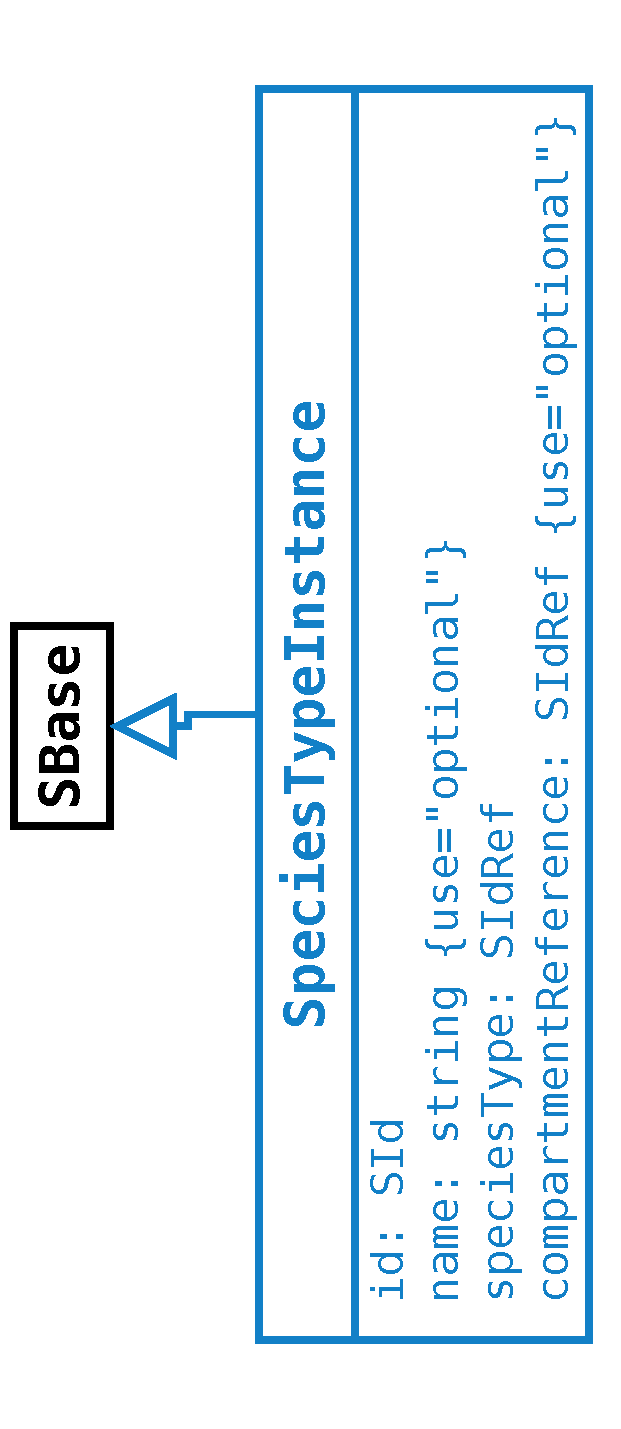
\includegraphics[angle=-90, scale=0.31]{./figs/multi_004_speciesTypeInstance.pdf}
    \caption{The definition of the \SpeciesTypeInstance class}
  \label{fig:SpeciesTypeInstance}
  \end{center}
\end{figure}

%-----------------------------------------------------------------------------------
\subsubsection{The \idAtt\ and \nameAtt\ attributes}
\label{def:SpeciesTypeInstance:idAndName}

The required \idAtt\ attribute, of type \SIdPT, serves to provide a way to identify a \speciesTypeInstance. Its value must be unique within its direct parent \speciesType. 

\class{SpeciesTypeInstance} also has an optional \nameAtt\ attribute of type \stringPT. 

%---------------------------------------------------------------
\subsubsection{The \speciesTypeAtt\ attribute}
\label{def:SpeciesTypeInstance:speciesType}

\class{SpeciesTypeInstance} has a required attribute \speciesTypeAtt, of type \SIdRefPT, is used to reference a \speciesType. 

%---------------------------------------------------------------
\subsubsection{The \compartmentReferenceAtt\ attribute}
\label{def:SpeciesTypeInstance:compartmentReference}

\class{SpeciesTypeInstance} has an optional attribute \compartmentReferenceAtt, of type \SIdRefPT, can be used to indicate which sub-compartment in a composite \compartment\ the \speciesTypeInstance\ is located in. 

For example, a compartment \val{cA} has two sub-compartments \val{cB1} (referenced by compartmentReference \val{crB1}) and \val{cB2} (referenced by compartmentReference \val{crB2}) of the same compartment type \val{cB}. A speciesType \val{stA} has two speciesTypeInstances \val{stiB1} and \val{stiB2} of the same speciesType \val{stB}. The speciesType \val{stA} references the compartment \val{cA} and the speciesType \val{stB} references the compartment \val{cB}. The speciesTypeInstance \val{stiB1} is located in \val{cB1} via the compartmentReference \val{crB1} and the speciesTypeInstance \val{stiB2} is located in \val{cB2} via the compartmentReference \val{crB2}. The SBML code can be as follows:

\label{example:SpeciesTypeInstance_compartmentReference}
\exampleFile{./examples/speciesTypeInstance_compartmentReference.xml}

\clearpage

%-------------------------------------
\subsection{\class{SpeciesTypeComponentIndex}}
\label{def:SpeciesTypeComponentIndex}

\class{SpeciesTypeComponentIndex} provides a way to identify or index a \component\ within a \speciesType. A \class{SpeciesTypeComponentIndex} object can be referenced by other class objects, such as \InSpeciesTypeBond, \OutwardBindingSite, \SpeciesFeature or \SpeciesTypeComponentMapInProduct objects, which needs to identify a component in a particular \speciesType. 

\class{SpeciesTypeComponentIndex} is defined in \fig{fig:SpeciesTypeComponentIndex}. It has two required attributes, \idAtt, and \componentAtt, and an optional attribute \identifyingParentAtt.  Since \class{SpeciesTypeComponentIndex} is derived from \class{SBase}, it inherits the \token{sboTerm} and \token{metaid} attributes, as well as the optional children \class{Notes} and \class{Annotation} objects. 

\begin{figure}[htb]
  \begin{center}
    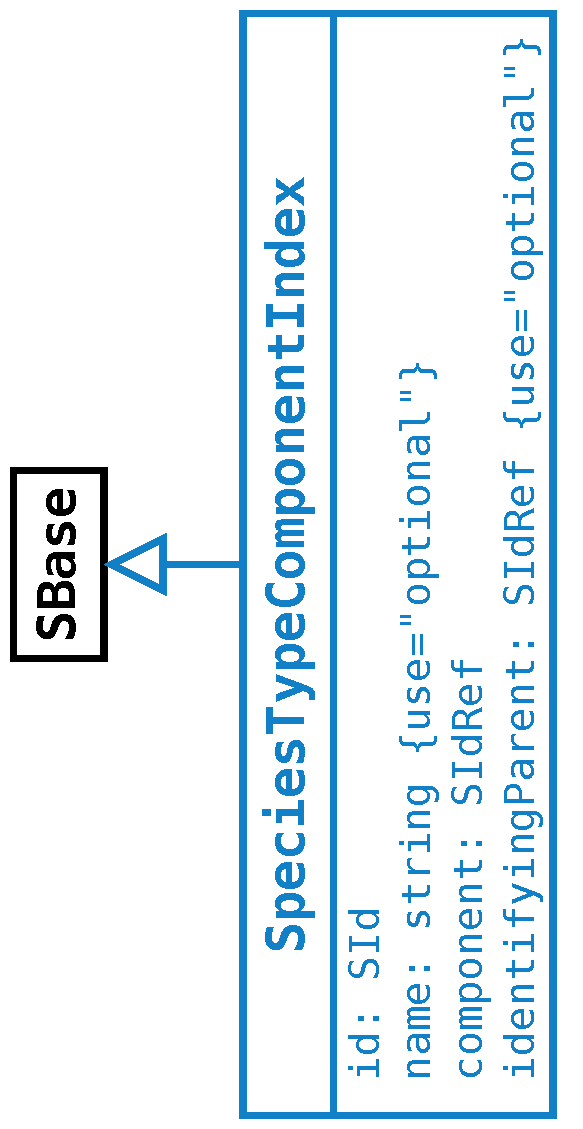
\includegraphics[angle=-90, scale=0.35]{./figs/multi_013_SpeciesTypeComponentIndex.pdf}
    \caption{The definition of the \SpeciesTypeComponentIndex class}
  \label{fig:SpeciesTypeComponentIndex}
  \end{center}
\end{figure}

See \sec{def:OutwardBindingSite:component} about how to use \SpeciesTypeComponentIndex in an \outwardBindingSite.

%------------------------------------
\subsubsection{The \idAtt\ attribute}
\label{def:SpeciesTypeComponentIndex:id}

The \idAtt\ attribute, of type \SIdPT, provides a way to identify a \speciesTypeComponentIndex. The value must be unique within the direct parent \speciesType.

%-------------------------------------------
\subsubsection{The \componentAtt\ attribute}
\label{def:SpeciesTypeComponentIndex:component}

The \componentAtt\ attribute, of type of \SIdRefPT, references a \speciesTypeInstance\ in the \speciesType, or the \speciesType\ itself. The value of this attribute can be the \idAtt\ of a \speciesTypeInstance\ or a \speciesTypeComponentIndex\ that is defined in the \speciesType\ of a \speciesTypeInstance. 

%-------------------------------------------------------
\subsubsection{The \identifyingParentAtt\ attribute}
\label{def:SpeciesTypeComponentIndex:identifyingParent}

The \componentAtt\ attribute itself may not be sufficient to uniquely reference a component in a \speciesType. The \identifyingParentAtt\ attribute provides assistance for the identification of a \componentWR. It references a parent of the component and the value can be the \idAtt\ of an object of \SpeciesTypeInstance, \SpeciesTypeComponentIndex or \SpeciesType.

This example illustrates the use of the \identifyingParentAtt\ attribute. There are three speciesTypes \val{stA}, \val{stB} and \val{stC}. The speciesType \val{stB} contains two speciesTypeInstances \val{C1} and \val{C2} of the same speciesType \val{stC}. The speciesType \val{stA} contains two speciesTypeInstances \val{B1} and \val{B2} of the same speciesType \val{stB}. The speciesType \val{A} may be required to index every \val{C1} and \val{C2} by its \ListOfInSpeciesTypeBonds child or referencing \token{species}. The following SBML code demonstrates how to do the indexing with assistance from the \identifyingParentAtt\ attribute.  

\exampleFile{./examples/SpeciesTypeComponentIndex_identifyingParent.xml}

In the speciesType \val{stA}, \val{B1C1} identifies the \val{C1} in \val{B1} and \val{B2C1} identifies the \val{C1} in \val{B2}. Similarly, \val{B1C2} identifies the \val{C2} in \val{B1} and \val{B2C2} identifies \val{C2} in \val{B2}.

%------------------------------------------------------
\subsubsection{Reference a \component\ in a \speciesType\ or a \species}
\label{def:SpeciesType:component}

In the Multi package, a component of a \speciesType\ may be a \speciesTypeInstance\ in the \speciesType\ or the \speciesType\ itself. This permits, for example, to define the \bindingStatusAtt\ of a binding site which may be a \speciesTypeInstance\ in a \species\ or a \speciesType\ directly referenced by a \species. The second case will be to reference a \speciesFeatureType\ of a \speciesTypeInstance\ in a \speciesType\ or a \speciesType\ itself. 

In many cases, to reference a component,  the \idAtt\ of the \component\ will be sufficient and it is not necessary to create an index (\speciesTypeComponentIndex). The example in \sec{def:SpeciesTypeComponentIndex:identifyingParent} illustrates two equivalent ways to reference a component, for example, the \val{B1} component in the \val{stA} speciesType. The creation of a \speciesTypeComponentIndex\ cannot be avoided when a \speciesType\ (indirectly) has two \speciesTypeInstances\ that have the same \idAtt.

\clearpage


%-------------------------------------
\subsection{\class{InSpeciesTypeBond}}
\label{def:InSpeciesTypeBond}

An \class{InSpeciesTypeBond} object defines a bond existing within a \speciesType. The bond therefore exists in every \species\ that references the \speciesType. 

\class{InSpeciesTypeBond} is defined in \fig{fig:InSpeciesTypeBond}. It has two optional attributes, \idAtt\ and \nameAtt, and two required attributes, \bindingSiteOneAtt\ and \bindingSiteTwoAtt.  Since \class{InSpeciesTypeBond} is derived from \class{SBase}, it inherits the \token{sboTerm} and \token{metaid} attributes, as well as the optional children \class{Notes} and \class{Annotation} objects. 

\begin{figure}[htb]
  \begin{center}
\ifpdf
    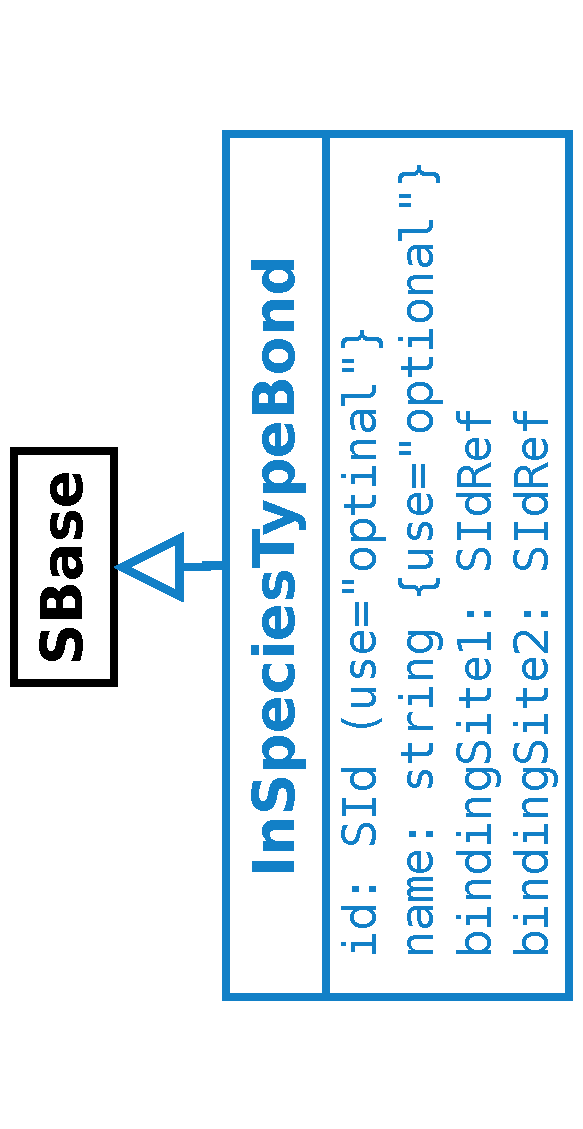
\includegraphics[angle=-90, scale=0.27]{./figs/multi_006_InSpeciesTypeBond.pdf}
\fi
    \caption{The definition of the \InSpeciesTypeBond class}
  \label{fig:InSpeciesTypeBond}
  \end{center}
\end{figure}

%-------------
\subsubsection{The \idAtt\ and \nameAtt\ attributes}
\label{def:InSpeciesTypeBond:idAndName}
%-------------

The optional \idAtt\ attribute, of type \SIdPT, provides a way to identify an \inSpeciesTypeBond. If present, the value of the \idAtt\ attribute must be unique within its directly parent \speciesType.

\class{InSpeciesTypeBond} also has an optional \nameAtt\ attribute, of type \stringPT. 

%-------------
\subsubsection{The \bindingSiteOneAtt\ and \bindingSiteTwoAtt\ attributes}
\label{def:InSpeciesTypeBond:bindingSites}
%-------------

\class{InSpeciesTypeBond} has two required attributes, \bindingSiteOneAtt\ and \bindingSiteTwoAtt, both of type \SIdRefPT, used to reference a pair of binding sites of the \InSpeciesTypeBond object in a \speciesType. The referenced identifiers of the binding sites can be the \idAtt s of the \speciesTypeInstances\ (binding sites), or the \idAtt s of the \objFont{speciesTypeComponent\-Indexes} indexing the binding sites  and the ultimately referenced components must be the \BindingSiteSpeciesType objects. Obviously, \bindingSiteOneAtt\ and \bindingSiteTwoAtt\ must not reference the same \BindingSiteSpeciesType object. 

\clearpage

%--------------------------------------------
\subsection{Uniqueness of \class{SpeciesType} definitions}
\label{def:SpeciesType:Uniqueness}
%--------------------------------------------

In some special cases, it may be possible to define a \speciesType\ in multiple equivalent ways. 

\fig{fig:SpeciesTypeUniqueness} shows an example of a \speciesType\ constructed in two different formats. The two \val{st\_x} speciesTypes in the diagram can be the results of different reaction paths, but they are equivalent and define the same \speciesType.

\begin{figure}[htb]
  \begin{center}
    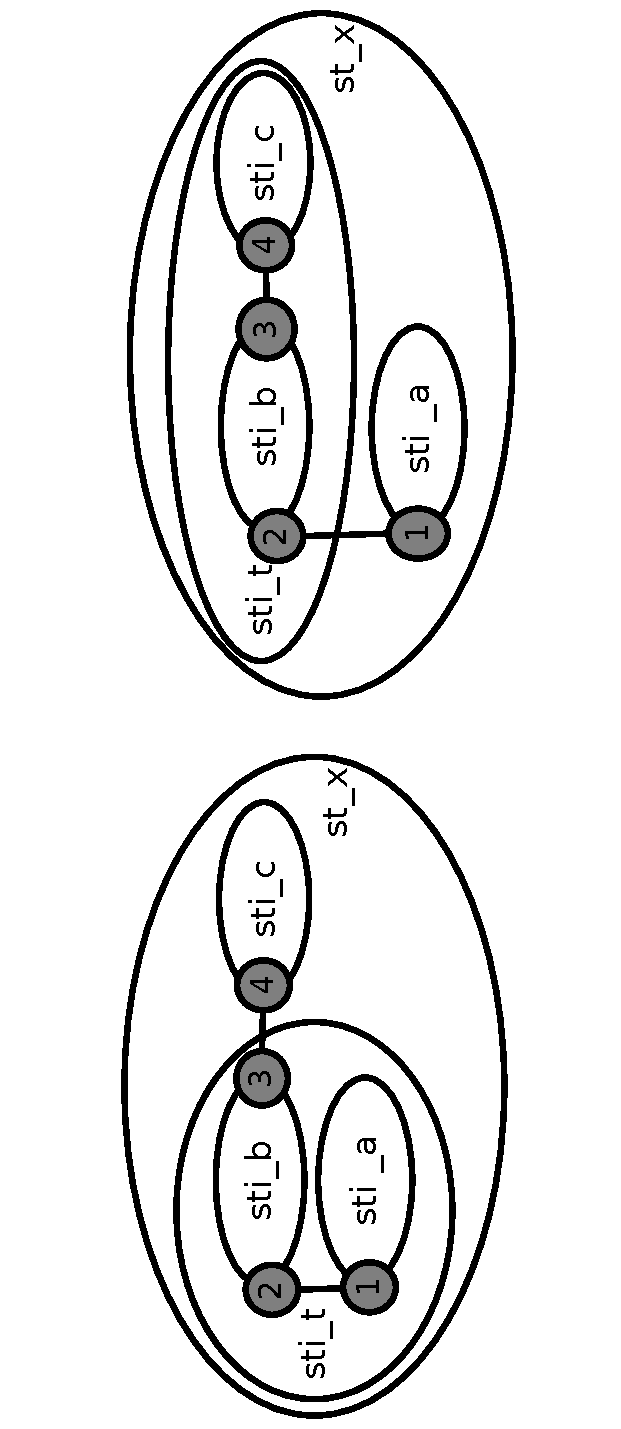
\includegraphics[angle=-90, scale=0.35]{./figs/diagram_SpeciesTypeUniqueness.pdf}
    \caption{Different formats of the same \speciesType}
    \label{fig:SpeciesTypeUniqueness}
  \end{center}
\end{figure}

Construct 1: The definition of speciesType \val{st\_x} on the left in \fig{fig:SpeciesTypeUniqueness}.
\exampleFile{./examples/SpeciesTypeUniquenessExample1.xml}

Construct 2: The definition of speciesType \val{st\_x} on the right in \fig{fig:SpeciesTypeUniqueness}.
\exampleFile{./examples/SpeciesTypeUniquenessExample2.xml}

This kind of ambiguity cannot be avoided for \speciesTypes\ involving more than two subcomponents connected by \inSpeciesTypeBonds, for example, the \speciesType\ referenced by the product \species\ in an association \reaction. It is up to the modeler (parser) to identify whether the two \speciesTypes\ such as those in the example above are identical.

\clearpage

%------------------------------------
\subsection{\class{Species}}
\label{def:ExSpecies}

A \species\ in \SbmlLevelThreeCore\ refers a pool of entities. A \species\ in the Multi package is extended from a pool to a template or pattern which multiple pools may map to. An extended \species\ can reference a \speciesType\ that provides the backbone for the \species\ such as \components\ (including \bindingSites) and \speciesFeatureTypes. When referencing a \speciesType, a \species\ can be further defined with regard to the binding statuses of its \outwardBindingSites\ and the \speciesFeatures. With the options to have variable values selected, such as \val{either} for the \bindingStatusAtt\ attribute and multiple \possibleSpeciesFeatureValues\ for a \speciesFeature, an extended \species\ can work as a template or pattern how \species\ participate in \reactions.  

The extension of the \Species class is illustrated in \fig{fig:ExSpecies}. The extended \ExSpecies class has a new optional attribute \speciesTypeAtt, and two extra optional \ListOfOutwardBindingSites and \ListOfSpeciesFeatures children. A \species\ may have a \listOfOutwardBindingSites\ child and/or a \listOfSpeciesFeatures\ child only when its \speciesTypeAtt\ attribute has been defined.

\begin{figure}[htb]
  \begin{center}
    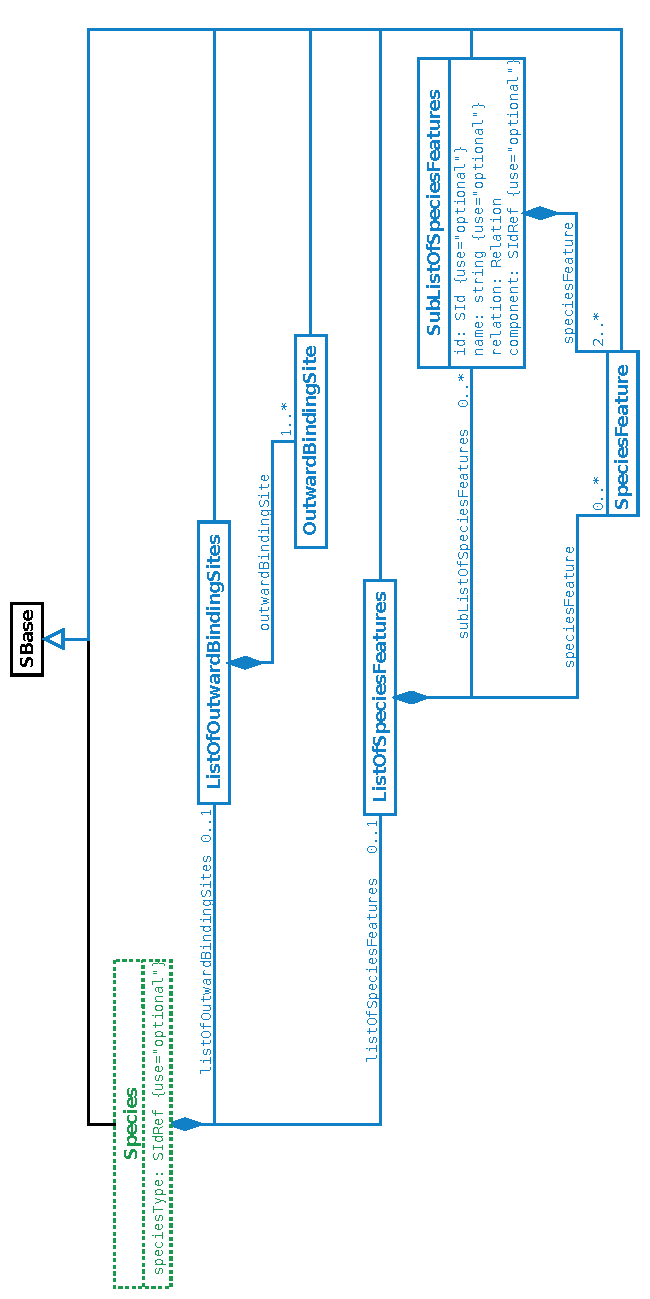
\includegraphics[angle=-90, scale=0.75]{./figs/multi_007_Species.pdf}
    \caption{The extension of the \ExSpecies class}
  \label{fig:ExSpecies}
  \end{center}
\end{figure}

%-------------
\subsubsection{The \speciesTypeAtt\ attribute}
\label{def:Species:speciesType}
%-------------

The optional attribute \speciesTypeAtt, of type \SIdRefPT, references a \SpeciesType object. 
 
%-------------------------------------
\subsubsection{\class{ListOfOutwardBindingSites}}
\label{def:ListOfOutwardBindingSites}

\class{ListOfOutwardBindingSites} is defined in \fig{fig:ExSpecies}, and can only be defined when the \speciesTypeAtt\ attribute is defined. If present, it must have one or more \OutwardBindingSite children.  Since \class{ListOfOutwardBindingSites} is derived from \class{SBase}, it inherits the \token{sboTerm} and \token{metaid} attributes, as well as the optional children \class{Notes} and \class{Annotation} objects. 

\noticeFont{Note: \notice \\
\label{note:outwardBindingSite:dontcare}
The \listOfOutwardBindingSites\ of a \species\ is not necessary to list all the \outwardBindingSites\ (the binding sites not involved in any \inSpeciesTypeBond) defined by the referenced \speciesType. If an \outwardBindingSite\ is not listed in the \listOfOutwardBindingSites, the value of its \bindingStatusAtt\ is \val{either}, in other words, the binding site is in a \val{don't care} state.
}

%-------------------------------------
\subsubsection{\class{ListOfSpeciesFeatures}}
\label{def:ListOfSpeciesFeatures}

\class{ListOfSpeciesFeatures} is defined in \fig{fig:ExSpecies}, and can only be defined when the \speciesTypeAtt\ attribute is defined. If present, it must have one or more children. A child can be a \SpeciesFeature object, or a \subListOfSpeciesFeatures, which is a \class{ListOfSpeciesFeatures} object.   

\ListOfSpeciesFeatures has an optional attribute \relationAtt, of type \RelationPTWC, to define the logic relationship among its children. The \relationAtt\ attribute can not be defined if a \listOfSpeciesFeatures\ has only one child, and it must be defined if the \listOfSpeciesFeatures\ has more than one children. 

\noticeFont{Note: \notice \\
\label{note:speciesFeature:dontcare}
The \listOfSpeciesFeatures\ of a \species\ does not have to cover all the \speciesFeatures\ corresponding to all \speciesFeatureTypes\ (see \sec{def:SpeciesFeatureType}) of every \component\ defined by the referenced \speciesType. If a \speciesFeatureType\ is defined and there is no \speciesFeature\ explicitly referencing it, the \species\ has an implicit \speciesFeature\ having all the \listOfPossibleSpeciesFeatureValues\ and \val{or} relationships between them. In other words, the implicit \speciesFeature\ has a \val{don't care} state for the \species.
}

 Since \class{ListOfSpeciesFeatures} is derived from \class{SBase}, it inherits the \token{sboTerm} and \token{metaid} attributes, as well as the optional children \class{Notes} and \class{Annotation} objects. 

The example at \sec{def:SpeciesFeature:Example} illustrates the usage of the \class{ListOfSpeciesFeatures} class.

\clearpage

%-------------------------------------
\subsection{\class{OutwardBindingSite}}
\label{def:OutwardBindingSite}

\class{OutwardBindingSite} is defined in \fig{fig:OutwardBindingSite}. It has two required attributes, \bindingStatusAtt\ and \componentAtt. A \bindingSite\ not involved in any \InSpeciesTypeBond object in the \speciesType\ referenced by a \species\ is an \outwardBindingSite.  Since \class{OutwardBindingSite} is derived from \class{SBase}, it inherits the \token{sboTerm} and \token{metaid} attributes, as well as the optional children \class{Notes} and \class{Annotation} objects. 

\begin{figure}[htb]
  \begin{center}
    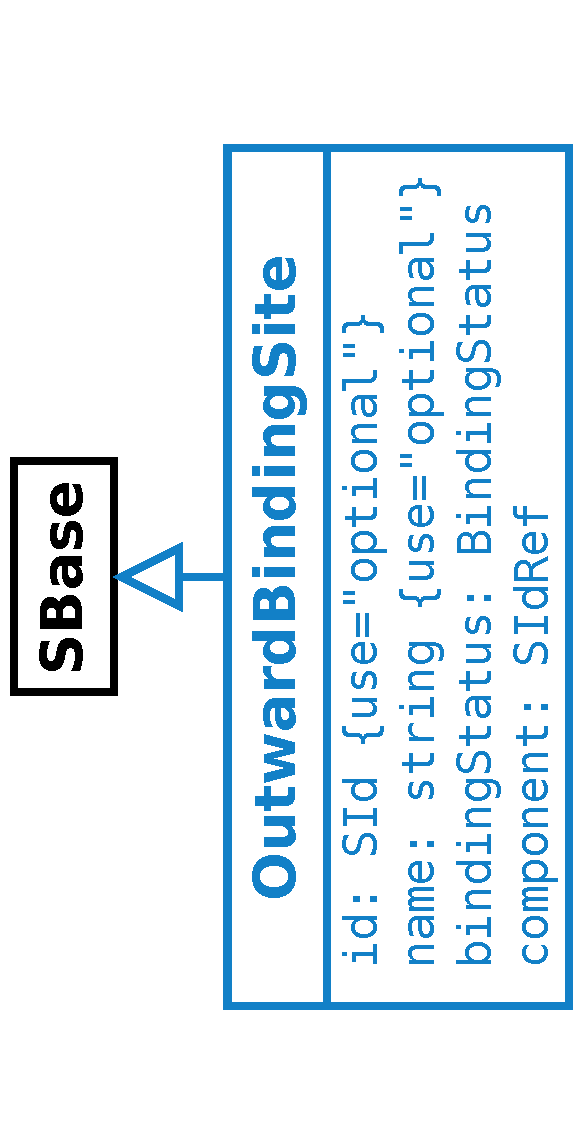
\includegraphics[angle=-90, scale=0.24]{./figs/multi_008_OutwardBindingSite.pdf}
    \caption{The definition of the \OutwardBindingSite class}
  \label{fig:OutwardBindingSite}
  \end{center}
\end{figure}

%-----------------------------------------------
\subsubsection{The \bindingStatusAtt\ attribute}
\label{def:OutwardBindingSite:bindingStatus}

The \bindingStatusAtt\ attribute takes a value of type \BindingStatusPTWC.

%-------------------------------------------
\subsubsection{The \componentAtt\ attribute}
\label{def:OutwardBindingSite:component}

The \componentAtt\ attribute, of type \SIdRefPT, references a \component\ which  ultimately reference a \BindingSiteSpeciesType object. The attribute value must be the identifier of a \SpeciesTypeInstance, \SpeciesTypeComponentIndex or \SpeciesType object.  

There are three scenarios for the \componentAtt\ attribute to have the value of an identifier of \SpeciesType, \SpeciesTypeInstance, or \SpeciesTypeComponentIndex respectively.

\begin{enumerate}[label=(\arabic*)]
 \item When a \species\ references a simple \bindingSiteSpeciesType, the value of the \componentAtt\ attribute of the \outwardBindingSite\ of the \species\ can only be the \idAtt\ of the referenced \speciesType.
 \item When a \species\ references a \speciesType\ with a \speciesTypeInstance\ being a binding site (have an \idAtt\ of \BindingSiteSpeciesType as its \speciesTypeAtt\ attribute) and the \idAtt\ of the \speciesTypeInstance\ can
identify the binding site within the \speciesType\ (referenced by the \species) unambiguously, and therefore, the value of the \componentAtt\ attribute of an \outwardBindingSite\ of the \species\ can be the \idAtt\ of the \speciesTypeInstance.
  \item When a \species\ references a \speciesType\ with a \speciesTypeInstance\ being a binding site (directly or indirectly) and \idAtt\ of the \speciesTypeInstance\ can NOT identify the binding site without ambiguity, an \idAtt\  of \SpeciesTypeComponentIndex can be used as the value of the \componentAtt\ attribute of an \outwardBindingSite of the \species.
\end{enumerate}

%----------------------
\subsubsection{Example}

\begin{figure}[htb]
  \begin{center}
    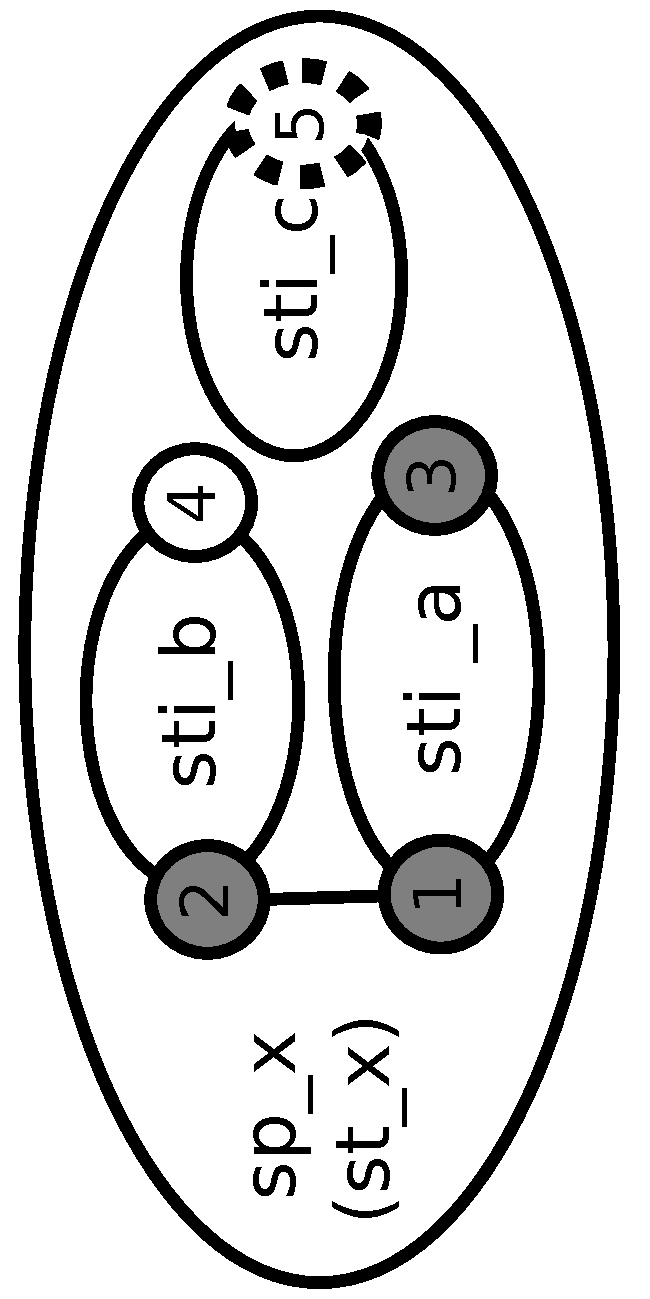
\includegraphics[angle=-90, scale=0.18]{./figs/diagram_OutwardBindingSite.pdf}
    \caption{An example of \OutwardBindingSite}
    \label{fig:OutwardBindingSiteExample}
  \end{center}
\end{figure}

\fig{fig:OutwardBindingSiteExample} illustrates the usage of the \OutwardBindingSite class. Species \val{sp\_x} references speciesType \val{st\_x}, which has three speciesTypeInstances \val{sti\_a}, \val{sti\_b} and \val{sti\_c}. SpeciesTypeInstance \val{sti\_a} has bindingSites \val{\_1} and \val{\_3}, speciesTypeInstance \val{sti\_b} has bindingSites \val{\_2} and \val{\_4}, and speciesTypeInstance \val{sti\_c} has bindingSite \val{\_5}. The \inSpeciesTypeBond\ in \val{st\_x} involves two bindingSites \val{\_1} and \val{\_2}. The other three bindingSites, \val{\_3}, \val{\_4} and \val{\_5}, in the species \val{sp\_x} are \outwardBindingSites. The outwardBindingSite \val{\_3} is \val{bound} (filled circle with solid line in the diagram), the outwardBindingSite \val{\_4} is \val{unbound} (empty circle with solid line) and the outwardBindingSite \val{\_5} has binding status \val{either} (empty circle with dotted line). The corresponding SBML code would be as follows:

\exampleFile{./examples/code_009_OutwardBindingSiteExample.xml}

\clearpage

%-------------------------------------
\subsection{\class{SpeciesFeature}}
\label{def:SpeciesFeature}

\class{SpeciesFeature} is defined in \fig{fig:SpeciesFeature}.  It has two optional attributes, \idAtt\ and \componentAtt, two required attributes, \speciesFeatureTypeAtt\ and \occurAtt, and a required child \listOfSpeciesFeatureValues. Since \class{SpeciesFeature} is derived from \class{SBase}, it inherits the \token{sboTerm} and \token{metaid} attributes, as well as the optional children \class{Notes} and \class{Annotation} objects. \class{SpeciesFeature} serves to define the state of a \component\ in a \species\ by selecting values from the \listOfPossibleSpeciesFeatureValues\ of the referenced \speciesFeatureType. 

\begin{figure}[htb]
  \begin{center}
    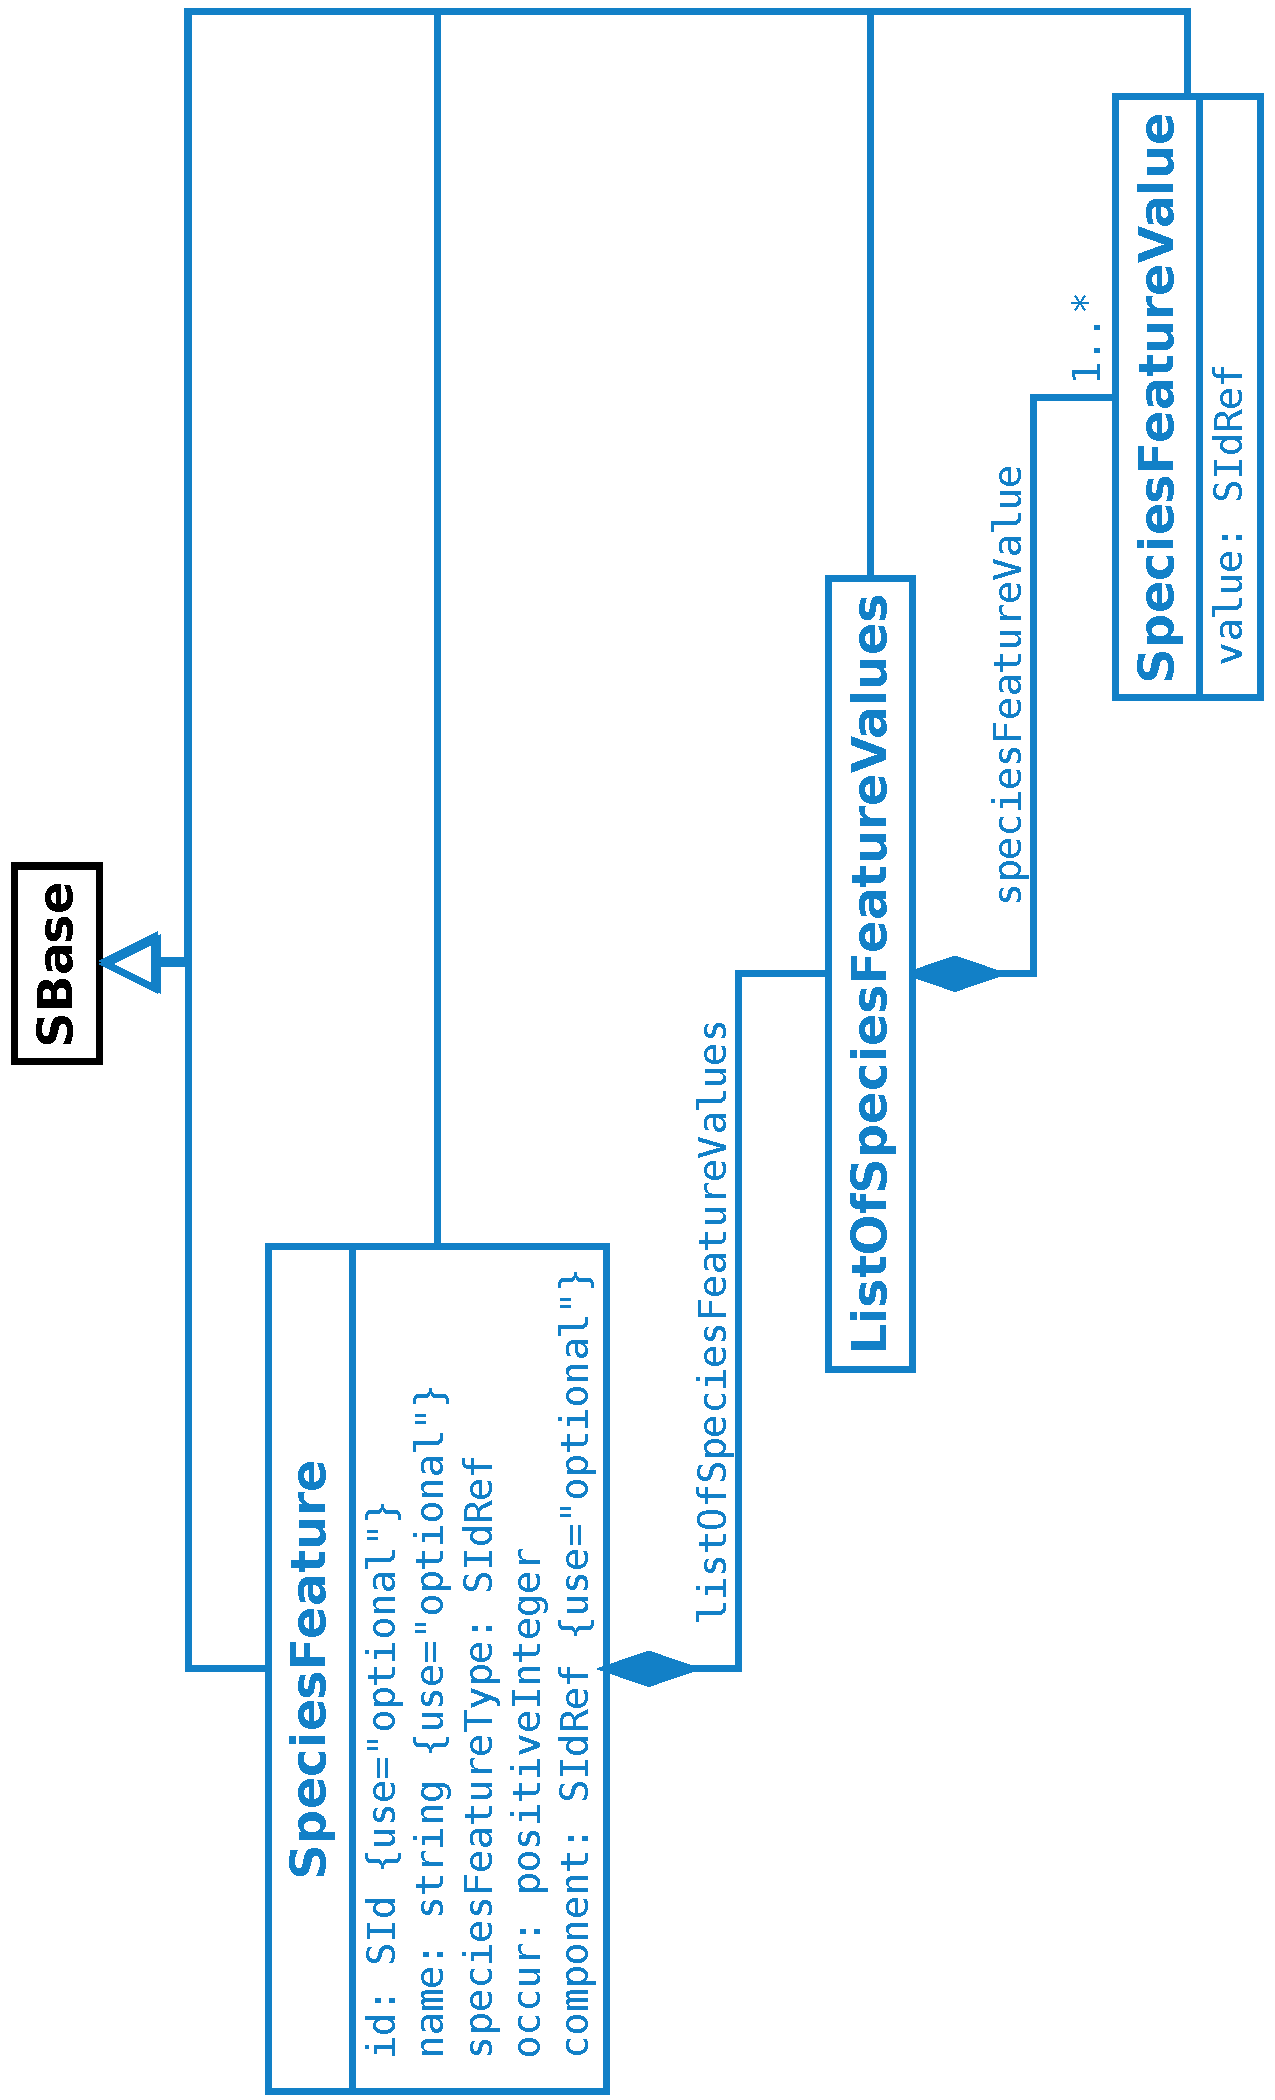
\includegraphics[angle=-90, scale=0.35]{./figs/multi_009_SpeciesFeature.pdf}
    \caption{The definitions of the \SpeciesFeature class and the \SpeciesFeatureValue class}
  \label{fig:SpeciesFeature}
  \end{center}
\end{figure}


%-------------------------------------------------------
\subsubsection{The \idAtt\ attribute}
\label{def:SpeciesFeature:id}

The optional \idAtt\ attribute, of type \SIdPT, can serve to provide a way to identify a \speciesFeature. If present, the value must be unique within the \species.

%-------------------------------------------------------
\subsubsection{The \speciesFeatureTypeAtt\ attribute}
\label{def:SpeciesFeature:speciesFeatureType}

\class{SpeciesFeature} has a required attribute \speciesFeatureTypeAtt, of type \SIdRefPT, used to reference a \objFont{speciesFeature\-Type}.

%---------------------------------------
\subsubsection{The \occurAtt\ attribute}
\label{def:SpeciesFeature:occur}

\class{SpeciesFeature} has a required attribute \occurAtt, of type of \positiveIntegerPT, used to define the number of instances of the referenced \speciesFeatureType. 

The value of the \occurAtt\ attribute can not be larger than the \occurAtt\ of the referenced \speciesFeatureType. When a \speciesFeatureType\ has multiple instances (\speciesFeatureType's \occurAtt\ > \val{1}), the \speciesFeature's \occurAtt\ attribute provides a way for a \species\ to define the instances of the \speciesFeatureType\ differently. 

For example, in a \speciesType, speciesFeatureType \val{ftA} has \occurAtt=\val{2} and two possibleSpeciesFeatureValues \val{fva1} and \val{fva2}. A \species\ referencing the \speciesType\ can be defined to have two speciesFeatures \val{sfA1} and \val{sfA2} both referencing \val{ftA}. The speciesFeature \val{sfA1} has \occurAtt=\val{1} and its value is \val{fva1}. The speciesFeature \val{sfA2} has \occurAtt=\val{1} and its value is \val{fva2}.

If the \occurAtt\ of a \speciesFeature\ is less than the \occurAtt\ of the referenced \speciesFeatureType, the rest of the unspecified instances of the \speciesFeatureType\ are in \val{don't care} state which means that the value of an unspecified instance can be any from the \listOfPossibleSpeciesFeatureValues. 

For example, in a \speciesType, a speciesFeatureType \val{phosphorylation} has two possibleSpeciesFeatureValues \val{phosphorylated} and \val{unphosphorylated} and the \occurAtt\ is \val{5}. A \species\ referencing the \speciesType\ can be defined to have a \speciesFeature\ of the \val{phosphorylation} with the value of \val{phosphorylated} and the \occurAtt\ of \val{1}. Then, the \species\ is a pattern \species\ with at least one \val{phosphorylated} site (the other four \val{phosphorylation} sites are in \val{don't care} state). (See the example in \sec{def:SpeciesFeatureChange:Example}.) This pattern \species\ can be mapped by anyone of the \fullydefinedspeciesWC\ of the same type and with any of \val{1} to \val{5} phosphorylated sites. 

%-------------------------------------------
\subsubsection{The \componentAtt\ attribute}
\label{def:SpeciesFeature:component}

The optional \componentAtt\ attribute, of type \SIdRefPT, can be used to indicate which \componentWR\ of a \species\ the \speciesFeature\ belongs to. It is required when the \component\ can not be identified only based on the\\
\speciesFeatureTypeAtt\ attribute.


%------------------------------------------------
\subsubsection{\class{ListOfSpeciesFeatureValues}}
\label{def:ListOfSpeciesFeatureValues}

\class{ListOfSpeciesFeatureValues} is defined in \fig{fig:SpeciesFeature}, and must have one or more \SpeciesFeatureValue children. If a \listOfSpeciesFeatures\ has multiple \speciesFeatureValues, the interpretation of the relationship between them is \val{or}. Since \class{ListOfSpeciesFeatureValues} is derived from \class{SBase}, it inherits the \token{sboTerm} and \token{metaid} attributes, as well as the optional children \class{Notes} and \class{Annotation} objects.

%-------------------------------------
\subsubsection{\class{SpeciesFeatureValue}}
\label{def:SpeciesFeatureValue}

\class{SpeciesFeatureValue} is defined in \fig{fig:SpeciesFeature}. A \speciesFeatureValue\ serves to specify a value for a \speciesFeature\ to select from the \listOfPossibleSpeciesFeatureValues\ defined in the referenced \speciesFeatureType. The \class{SpeciesFeatureValue} class has only one attribute \valueAtt\, of type \SIdRefPT, used to reference a \PossibleSpeciesFeatureValue object. Since \class{SpeciesFeatureValue} is derived from \class{SBase}, it inherits the \token{sboTerm} and \token{metaid} attributes, as well as the optional children \class{Notes} and \class{Annotation} objects. 


%----------------------------------------------------------------------------
\subsubsection{Example}
\label{def:SpeciesFeature:Example}
%----------------------------------------------------------------------------

\fig{fig:ListOfSpeciesFeaturesExample} is an example \speciesType\ to illustrate the usage of the \ListOfSpeciesFeatures and \SpeciesFeature classes. SpeciesType \val{st\_A} has a speciesFeatureType \val{fA} which has two possibleSpeciesFeatureValues \val{fa1} and \val{fa2}. The speciesType \val{st\_A} also has two children speciesTypeInstances \val{sti\_B} and \val{sti\_C}, which have speciesFeatureTypes \val{fB} and \val{fC} respectively. The speciesFeatureType \val{fB} has possibleSpeciesFeatureValues \val{fb1} and \val{fb2}, and the speciesFeatureType \val{fC} has \val{fc1} and \val{fc2}. Here are several ways to construct the listOfSpeciesFeatures of a \species\ referencing the speciesType \val{st\_A}:
\begin{itemize}
 \item 
   listOfSpeciesFeatures (relation=\val{and}, children=\val{fa1}, \val{fb1},  \val{fc1}) is a state: \\ 
   \val{[fa1] and [fb1] and [fc1]} 
 \item 
   listOfSpeciesFeatures (relation=\val{or}, children=\\
   \parindent 20pt 
   \indent subListOfSpeciesFeatures (relation=\val{and}, children=\val{fa1}, \val{fb1},  \val{fc1}),\\
   \indent subListOfSpeciesFeatures (relation=\val{and}, children=\val{fa2}, \val{fb2},  \val{fc2})\\
    ) is a state: \\ 
    \val{[fa1] and [fb1] and [fc1]} or \val{[fa2] and [fb2] and [fc2]}
 \item 
   listOfSpeciesFeatures (relation=\val{and}, children=\\
   \parindent 20pt 
   \indent \val{fa1},\\
   \indent subListOfSpeciesFeatures (relation=\val{not}, children=\val{fb1},  \val{fc1})\\
 ) is a state: \\ 
   \val{[fa1] and [fb1] and [fc2]} or 
   \val{[fa1] and [fb2] and [fc2]} or 
   \val{[fa1] and [fb2] and [fc1]}
\end{itemize}

\begin{figure}[htb]
  \begin{center}
    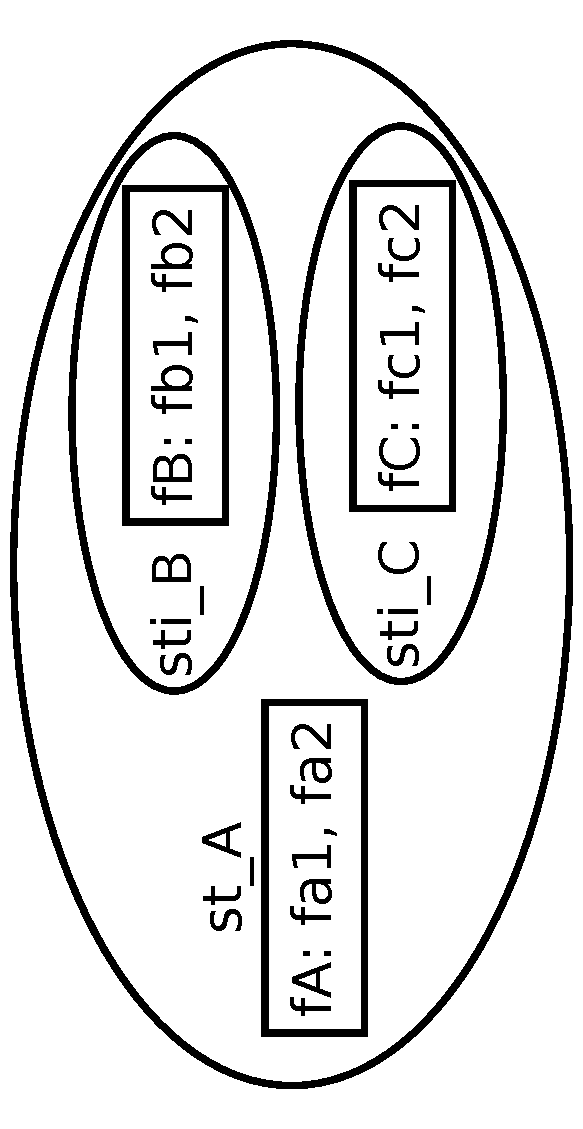
\includegraphics[angle=-90, scale=0.26]{./figs/diagram_ListOfSpeciesFeatures.pdf}
    \caption{An example \speciesFeatureType\ to illustrate the usage of the \ListOfSpeciesFeatures class and the \SpeciesFeature class}
  \label{fig:ListOfSpeciesFeaturesExample}
  \end{center}
\end{figure}

The SBML code can be as follows and the species \val{sp\_A1}, \val{sp\_A2} and \val{sp\_A3} contain the tree \objFont{listOfSpecies\-Features} above respectively.

\exampleFile{./examples/code_SpeciesFeatureExample.xml}

\clearpage

%------------------------------------------
\subsection{\Fullydefinedspecies\ and the mapping to \val{pattern} \species}
\label{def:Species:FullyDefined}

An extended \ExSpecies object functions as a template or a pattern which allows multiple pools of entities to map to it. A \species\ is \val{fully defined} if there is only one pool mapping to it. A \fullydefinedspecies\ can be considered the same as a SBML core \species, and can be initialized with the \initialAmountAtt\ attribute, or the \initialConcentrationAtt\ attribute, or via an \InitialAssignment object. In the Multi package, a \species\ is \fullydefined\ if the following conditions are fulfilled.

\begin{itemize}
 \item All \outwardBindingSites\ must be free (\bindingStatusAtt=\val{unbound}), since \val{bound} sites imply that there is a non-specified binding partner.
 \item Each \speciesFeature\ occurrence can only have one \speciesFeatureValue, and every occurrences of every \speciesFeatureTypes\ of every \components\ of the referenced \speciesType\ must be referenced by exactly one \speciesFeature\  occurrence.
 \item If applicable, only \val{and} values are allowed for the \relationAtt\ attributes of the \ListOfSpeciesFeatures objects.
 \item Only one single \SpeciesFeatureValue object is allowed for any \speciesFeature.
 \item The referenced \compartment\ can not be a \objFont{compartment type}, which means the value of the \isTypeAtt\ attribute of the referenced \compartment\ can only be \val{false}.
\end{itemize}

The mapping from a \fullydefinedspecies\ to a \val{pattern} species is implicit and can be inferred from the structure of the \species. For example, a speciesType \val{stA} has one \speciesFeatureType\ with two possibleSpeciesFeatureValues \val{v1} and \val{v2}. A species \val{spA1} references \val{stA} and has the \speciesFeature\ with the value of \val{v1}. Another species \val{spA} also references \val{stA} and has no \speciesFeature\ explicitly defined. Thus, the species \val{spA1} is a \fullydefinedspecies\ and can map to the \val{pattern} species \val{spA} because species \val{spA} has an implicit \speciesFeature\ which can take either value \val{v1} or value \val{v2} (see the note in \sec{note:speciesFeature:dontcare}).

\noticeFont{Note: \notice \\
\label{note:fullydefinedspecies:not}
Theoretically, using \val{not} and \val{or} can also result in a \fullydefinedspecies. For example, a \speciesType\ has two feature types \val{A} (\val{a1} and \val{a2} as possible values) and \val{B} (\val{b1} and \val{b2} as possible values). A \fullydefinedspecies\ referencing the \speciesType\ can be defined to have a feature of \val{[a1 and b1]}. Equivalently, the \species\ can also be defined to have \val{[not ([a1 and b2] or [a2 and b2] or [a2 and b1])]}. In the Multi package, the main reason to define \fullydefinedspecies\ is to initialize \species\ in a \model. Therefore, the definition for \fullydefinedspecies\ simply disallows \val{not} and \val{or} to make it easier for a modeler to define \fullydefinedspecies.
}

\clearpage

%------------------------------------
\subsection{\class{Reaction}}
\label{def:ExReaction}


\class{Reaction} itself in the Multi package is not extended, but it may use the Multi \ExSpecies\ objects to construct \reactions. The \class{Reaction} class in the Multi package can not only define the relations among pools (SBML core \species), but also the relations among patterns (Multi extended \species). Several related classes including \ExSimpleSpeciesReference and \ExSpeciesReference are extended to handle some issues specific to the Multi package. A new class, \IntraSpeciesReaction, is derived from \class{Reaction} to explicitly define those reactions within the same \ExSpecies\ object.

The changes under the \class{Reaction} class in the Multi package are illustrated in \fig{fig:ExReaction}. 

\begin{figure}[htb]
  \begin{center}
\ifpdf
    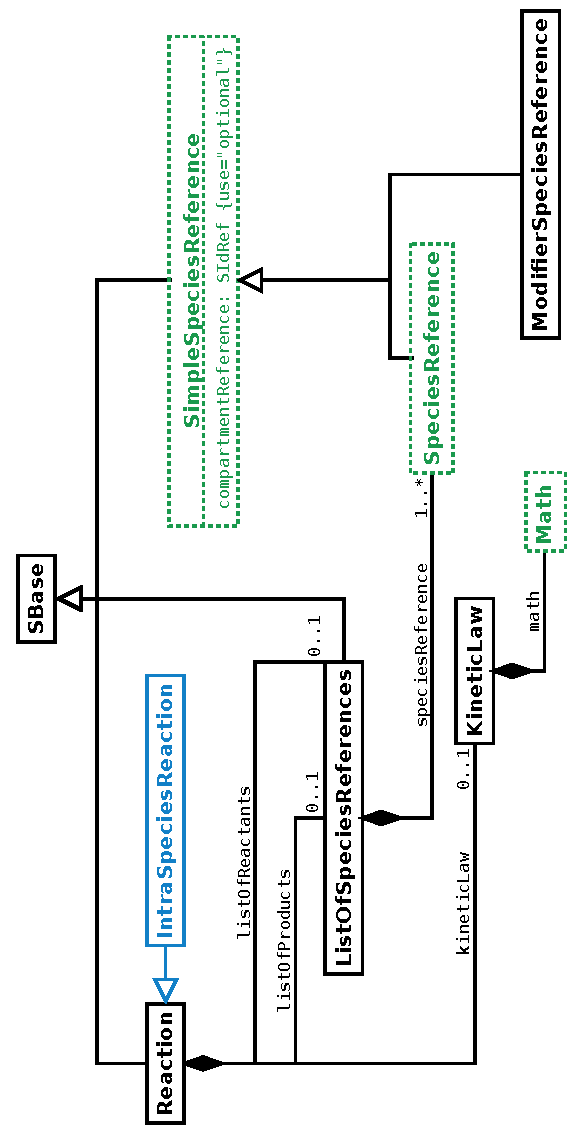
\includegraphics[angle=-90, scale=0.8]{./figs/multi_010_Reaction.pdf}
\fi
    \caption{The changes under the \ExReaction class including \IntraSpeciesReaction, \ExSimpleSpeciesReference, \ExSpeciesReference and \ExMath}
  \label{fig:ExReaction}
  \end{center}
\end{figure}

%------------------------------------
\subsection{\class{IntraSpeciesReaction}}
\label{def:IntraSpeciesReaction}

\class{IntraSpeciesReaction} is derived from \class{Reaction} for the \reactions\ happening within a \species\ (see the example \val{Extended Reaction class} at page 23  of the slides at HARMONY 2013 [\cite{ref:harmony2013}]).

A particular \reaction\ may happen within a \species\ as an \intraSpeciesReaction\ if the following conditions are fulfilled. 
\begin{itemize}
 \item The \reaction\ is either an association \reaction\ or a dissociation \reaction.
 \item If it is an association \reaction, each of the two reactant \species\ has at least one \outwardBindingSite\ free (\val{unbound}).
 \item If it is a dissociation \reaction, each of the two product \species\ has at least one \outwardBindingSite\ free (\val{unbound}).
\end{itemize}

\noticeFont{Note: \notice \\
\label{Note:IntraSpeciesReaction}
Technically, transformations are also reactions happening with one \species, but they do not have the ambiguity of association and dissociation \reactions. Therefore, transformation \reactions\ do not have to be defined as \intraSpeciesReactions.  
}

\clearpage

%------------------------------------
\subsection{Extended \class{SimpleSpeciesReference}}
\label{def:ExSimpleSpeciesReference}

The \SimpleSpeciesReference class is extended with a new optional attribute \compartmentReferenceAtt, of type \SIdRefPT, to reference a \compartmentReference. The \compartmentReferenceAtt\ attribute can serve to indicate which sub-compartment where an object of a class (\SpeciesReference or \ModifierSpeciesReference) inheriting \class{SimpleSpeciesReference} is located. 

This example illustrates the use of the \compartmentReferenceAtt\ attribute. A model has a compartment type \val{c} and a composite compartment type \val{cc} with two compartmentReferences \val{cr1} and \val{cr2} both referencing the \val{c} compartment type. Both species \val{spA} and \val{spM} reference the \val{c} compartment type. A reaction happens between two \val{spA} species from the two compartments respectively and results in a cross-compartment product. One condition for this reaction is that two \val{spM} species work as modifiers in the two \val{c} compartments respectively. The situation described here could correspond to interactions among species located on two adjacent membranes. Without the \compartmentReferenceAtt\ attribute in the \class{SimpleSpeciesReference} class, it is impossible to distinguish the two \val{spA} species as well as the two \val{spM} species. The SBML code can be as follows:

\exampleFile{./examples/code_015_SimpleSpeciesReference.xml}

\clearpage

%------------------------------------
\subsection{Extended \class{SpeciesReference}}
\label{def:ExSpeciesReference}

The \SpeciesReference class is extended from \SbmlLevelThreeCore\ and can establish \component\ mappings between the reactant \species\ and the product \species\ when the mappings can not be inferred from the \idAtt s of the \SpeciesTypeInstance objects. The \SpeciesReference class has an optional \ListOfSpeciesTypeComponentMapsInProduct child, as defined in \fig{fig:ExSpeciesReference}. Only a \reaction\ \product\ can contain the \ListOfSpeciesTypeComponentMapsInProduct child and it is not necessary to store the mappings again in the \reactants.

\begin{figure}[htb]
  \begin{center}
    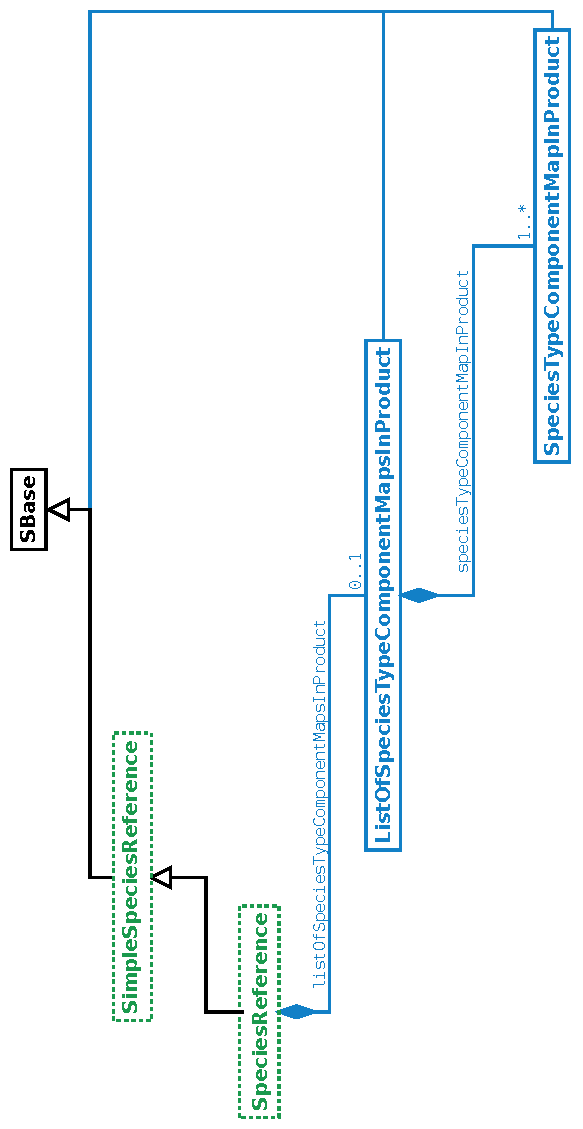
\includegraphics[angle=-90, scale=0.8]{./figs/multi_011_SpeciesReference.pdf}
    \caption{The extension of the \ExSpeciesReference class}
  \label{fig:ExSpeciesReference}
  \end{center}
\end{figure}

%------------------------------------
\subsubsection{\class{ListOfSpeciesTypeComponentMapsInProduct}}
\label{def:ListOfSpeciesTypeComponentMapsInProduct}

\class{ListOfSpeciesTypeComponentMapsInProduct} is defined in \fig{fig:ExSpeciesReference}. If present, it must have one or more \SpeciesTypeComponentMapInProduct children.  Since \class{ListOfSpeciesTypeComponentMapsInProduct} is derived from \class{SBase}, it inherits the \token{sboTerm} and \token{metaid} attributes, as well as the optional children \class{Notes} and \class{Annotation} objects. 

\clearpage

%-------------------------------------------------
\subsection{\class{SpeciesTypeComponentMapInProduct}}
\label{def:SpeciesTypeComponentMapInProduct}

\class{SpeciesTypeComponentMapInProduct} is defined in \fig{fig:SpeciesTypeComponentMapInProduct}.  Since \class{SpeciesTypeComponentMapInProduct} is derived from \class{SBase}, it inherits the \token{sboTerm} and \token{metaid} attributes, as well as the optional children \class{Notes} and \class{Annotation} objects. 

A \speciesTypeComponentMapInProduct\ defines the mapping between a \component\ in a reactant and a \component\ in a product.  The identifications of a \componentWR\ and the \speciesReference\ should be sufficient to identify the \component\ in the context of a \reaction. The attributes \reactantAtt\ and \reactantComponentAtt\ can identify the \component\ in a \reactant, and the \productComponentAtt\ attribute and the product storing the mapping information can identify the \component\ in a \product. 

\begin{figure}[htb]
  \begin{center}
    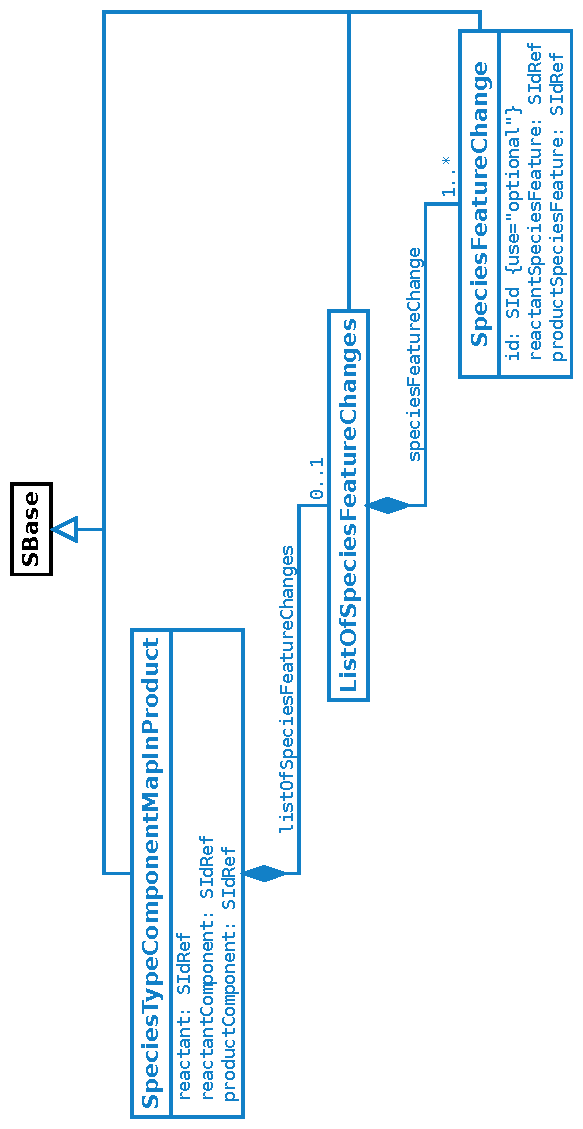
\includegraphics[angle=-90, scale=0.7]{./figs/multi_014_SpeciesTypeComponentMapInProduct.pdf}
    \caption{The definitions of the \SpeciesTypeComponentMapInProduct and \SpeciesFeatureChange classes}
  \label{fig:SpeciesTypeComponentMapInProduct}
  \end{center}
\end{figure}

 % this part, only wording has been changed, no ``real'' content change
%------------------------------------------
\subsubsection{The \reactantAtt\ attribute}
\label{def:SpeciesTypeComponentMapInProduct:reactant}

\class{SpeciesTypeComponentMapInProduct} has a required \reactantAtt\ attribute, of type \SIdRefPT, to reference the  \idAtt\ of a reactant \speciesReference\ in a \reaction.

%---------------------------------------------------
\subsubsection{The \reactantComponentAtt\ attribute}
\label{def:SpeciesTypeComponentMapInProduct:reactantComponent}

\class{SpeciesTypeComponentMapInProduct} has a required \reactantComponentAtt\ attribute, of type \SIdRefPT, to reference a \componentWR\ in a reactant \species. 

%--------------------------------------------------
\subsubsection{The \productComponentAtt\ attribute}
\label{def:SpeciesTypeComponentMapInProduct:productComponent}

\class{SpeciesTypeComponentMapInProduct} has a required \productComponentAtt\ attribute, of type \SIdRefPT, to reference a \componentWR\ in a product \species. 


%--------------------------------------------------
\subsubsection{\class{ListOfSpeciesFeatureChanges}}
\label{def:ListOfSpeciesFeatureChanges}

\class{SpeciesTypeComponentMapInProduct} also has an optional \ListOfSpeciesFeatureChanges child to explicitly define changes of \speciesFeatures\ in a \reaction. If present, it must have one or more \SpeciesFeatureChange children.  Since \class{ListOfSpeciesFeatureChanges} is derived from \class{SBase}, it inherits the \token{sboTerm} and \token{metaid} attributes, as well as the optional children \class{Notes} and \class{Annotation} objects. 

\clearpage

%----------------------------------------
\subsection{\class{SpeciesFeatureChange}}
\label{def:SpeciesFeatureChange}

\class{SpeciesFeatureChange} is defined in \fig{fig:SpeciesTypeComponentMapInProduct} and provides a way to specify how some of or all instances of a \speciesFeatureType\ to change. This class should only be used when the \occurAtt\ of the referenced \speciesFeatureType\ is larger than \val{1}. The parent \components\ of the changed \speciesFeatures\ are identified in the \SpeciesTypeComponentMapInProduct object. \class{SpeciesFeatureChange} has one optional attribute \idAtt\ and two required attributes, \reactantSpeciesFeatureAtt\ and \productSpeciesFeatureAtt. The \occurAtt\ attributes of the changed \speciesFeatures\ in \reactant\ and \product\ respectively must have the same value. 

 Since \class{SpeciesFeatureChange} is derived from \class{SBase}, it inherits the \token{sboTerm} and \token{metaid} attributes, as well as the optional children \class{Notes} and \class{Annotation} objects. 

%--------------------------------------------------------
\subsubsection{The \idAtt\ attribute}
\label{def:SpeciesFeatureChange:id}

The optional \idAtt\ attribute, of type \SIdPT, provides a way to identify a \speciesFeatureChange. 

%--------------------------------------------------------
\subsubsection{The \reactantSpeciesFeatureAtt\ attribute}
\label{def:SpeciesFeatureChange:reactantSpeciesFeature}

The \reactantSpeciesFeatureAtt\ attribute, of type \SIdRefPT, references a \speciesFeature\ in the reactant \componentWR\ in a reaction mapping.

%--------------------------------------------------------
\subsubsection{The \productSpeciesFeatureAtt\ attribute}
\label{def:SpeciesFeatureChange:productSpeciesFeature}

The \productSpeciesFeatureAtt\ attribute, of type \SIdRefPT, references a \speciesFeature\ in the product \componentWR\ in a reaction mapping.

%----------------------
\subsubsection{Example}
\label{def:SpeciesFeatureChange:Example}

Here is an example to illustrate the use of the \SpeciesFeatureChange class in a phosphorylation reaction. One among the five sites in a species is transformed from \val{unphosphorylated} to \val{phosphorylated} and the phosphorylation sites are defined as the referenced speciesFeatureType with \occurAtt=\val{5}. The SBML code can be as follows:

\exampleFile{./examples/SpeciesFeatureChangeExample.xml}

\clearpage

%---------------
\subsection{The \outwardBindingSites\ and \speciesFeatures\ in \val{don't care} state in a reaction \product}
\label{def:Reaction:dontcaredontchange}

An \outwardBindingSite\ is in \val{don't care} state if its \bindingStatusAtt\ is \val{either} or is not specified (also see \sec{def:ListOfOutwardBindingSites}). A \speciesFeature\ or an instance of a \speciesFeature\ (the \occurAtt\ of its \speciesFeatureType\ is larger than \val{1}) is in \val{don't care} state if it has all the \possibleSpeciesFeatureValues\ under its \objFont{species\-FeatureType}, or it is not specified in the \species\ (also see \sec{def:ListOfSpeciesFeatures}). 

For a \species\ as a \product\ in a reaction, if it has \val{don't care} \outwardBindingSites\ or \val{don't care} \objFont{species\-Features}, the interpretation of the \val{don't care} is \val{don't change}. In a \product, a \val{don't care} \objFont{outward\-BindingSite} has the same \bindingStatusAtt\ as the mapped \outwardBindingSite\ in the \reactant, and a \val{don't care} \speciesFeature\ or instance of a \speciesFeature\ has the same value as the mapped \speciesFeature\ or the mapped \speciesFeature\ instance in the \reactant.

For the phosphorylation example in \sec{def:SpeciesFeatureChange:Example}, the reactant species has one \val{unphosphorylated} site and four \val{don't care} sites, and the product species has one \val{phosphorylated} site and four {don't care} sites. The \val{phosphorylation} reaction can apply to the following \reactions\ of \fullydefinedspecies.
\begin{itemize}
 \item Reactant: a \species\ with \val{0} phosphorylated site and \val{5} unphosphorylated sites.
 
       Product: a \species\ with  \val{1} phosphorylated site and \val{4} unphosphorylated sites.
 \item Reactant: a \species\ with \val{1} phosphorylated site and \val{4} unphosphorylated sites.
 
       Product: a \species\ with  \val{2} phosphorylated sites and \val{3} unphosphorylated sites.
 \item Reactant: a \species\ with \val{2} phosphorylated sites and \val{3} unphosphorylated sites.
 
       Product: a \species\ with  \val{3} phosphorylated sites and \val{2} unphosphorylated sites.
 \item Reactant: a \species\ with \val{3} phosphorylated sites and \val{2} unphosphorylated sites.
 
       Product: a \species\ with  \val{4} phosphorylated sites and \val{1} unphosphorylated site.
 \item Reactant: a \species\ with \val{4} phosphorylated sites and \val{1} unphosphorylated site.
 
       Product: a \species\ with  \val{5} phosphorylated sites and \val{0} unphosphorylated site.
\end{itemize}

\clearpage

%---------------------------------------------------------
\subsection{Extended \objFont{ci} elements in \class{Math} objects}
\label{def:Reaction:Math:ci}

The Multi package extends the \token{ci} element in \class{Math} in \ExReaction with optional attributes \speciesReferenceAtt\ and \representationTypeAtt.

%--------------------------------------------------
\subsubsection{The \speciesReferenceAtt\ attribute}
\label{def:Reaction:Math:ci:speciesReference}

The optional \speciesReferenceAtt\ attribute, of type \SIdRefPT, can only be used when the content of the \objFont{ci} element is a \species\ \idAtt, or when the content of the \objFont{ci} element is a \speciesFeature\ \idAtt. The \speciesReferenceAtt\ attribute can identify which \species\ is referenced in a \reaction, and the \speciesReferenceAtt\ attribute must have a value of a \speciesReference\ \idAtt\ within the same reaction. 

If the \objFont{ci} content references a \species' \idAtt, the \idAtt\ represent the concentration of the \species. 

If the \objFont{ci} content references a \speciesFeature's \idAtt, the \idAtt\ represent the count of the \speciesFeature\ instances with the \speciesFeatureValue\ (also see \sec{def:SpeciesFeature:id}).  


The example in \sec{def:ExSimpleSpeciesReference} can be further extended with a block of \objFont{kineticLaw} in the \reaction\ to illustrate the use of the \speciesReferenceAtt\ attribute with a \species' \idAtt.

\exampleFile{./examples/ci_speciesReferenceAtt_species.xml}

Two \val{spA} \species\ and two \val{spM} \species\ are distinguished by the \val{r1} and \val{r2} \speciesReferences\ respectively. 


Here is another example to show the use of the \speciesReferenceAtt\ attribute for a \possibleSpeciesFeatureValue. This example is a simplified adaptation of published \smodels\ [\cite{ref:scaffoldProteinNature2010}, \cite{ref:yeastMSB2010}]. A \speciesType\ \val{stY} has 10 phosphorylation sites. A \species\ \val{Yu} referencing \speciesType\ \val{stY} can be phosphorylated by another \species\ \val{M} one site one time and the phosphorylation rate depends on the number of sites already phosphorylated in \species\ \val{Yu}. The SBML code can be as follows:

\label{def:Reaction:Math:ci:speciesReference:speciesFeature}
\exampleFile{./examples/ci_speciesReferenceAtt_speciesFeature.xml}

Any \fullydefinedspecies\ referencing \val{stY} with at least one unphosphorylated site maps to the species \val{Yu}. Any \fullydefinedspecies\ referencing \val{stY} with at least one phosphorylated site maps to the species \val{Yp}. The \speciesFeatureChange\ references speciesFeatures \val{fU} and \val{fP} and the value of \val{1} for both \occurAtt\ attributes of \val{fU} and \val{fP} indicates that one site is phosphorylated in the \reaction. The \code{<ci multi:speciesReference=}\val{r}\code{> P </ci>} depends on the \fullydefinedspecies\ mapping to the species \val{Yu} which is referenced by the speciesReference \val{r}. If the \fullydefinedspecies\ has 1 site phosphorylated, the \objFont{ci} is \val{1} in the math, similarly, \objFont{ci} is 2 for 2 phosphorylated sites, ...., \objFont{ci} is 9 for 9 phosphorylated sites.  

%--------------------------------------------------
\subsubsection{The \representationTypeAtt\ attribute}
\label{def:Reaction:Math:ci:representationType}

The optional \representationTypeAtt\ attribute, of type \RepresentationTypePTWC, can only be used when the content of the \objFont{ci} element is a \species' \idAtt\ or a \possibleSpeciesFeatureValue's \idAtt. The \representationTypeAtt\ and \speciesReferenceAtt\ attributes can both be used for the same \objFont{ci} element at the same time. 

The \representationTypeAtt\ attribute can only have the value of \val{sum} when the content of the \objFont{ci} is \species. The interpretation of such a \objFont{ci} element is the total concentration or amount of all \fullydefinedspeciesWC\ mapping to the referenced pattern \species.   

The \representationTypeAtt\ attribute can have the value of \val{numericValue} when the content of the \objFont{ci} is \possibleSpeciesFeatureValue\ and the \speciesReferenceAtt\ attribute must be defined. The interpretation of such a \objFont{ci} is the same as a \objFont{ci} element having a \objFont{parameter} which the \possibleSpeciesFeatureValue\ links via its \numericValueAtt\ attribute.   

The following example demonstrates the use of this attribute for \val{sum} of \species\ concentrations.

\begin{example}[style=latex]
    k1*Si/(k2+SUM(Si)) 
\end{example}

In this example, the \reactant\ \val{Si} is a pattern \species\ which may have multiple \fullydefinedspecies\ mapping to it, for example \species\ \val{S1}, \val{S2}, ..., \val{Sn}.  \val{SUM(Si)} is a function to calculate the total concentration of all \fullydefinedspecies\ mapping to \val{Si}. The \product\ can be another pattern \species\ \val{Pi}. The SBML code for the math expression can be as follows:

\exampleFile{./examples/ci_patternSpecies_sum.xml}

The math expressions for the individual \species\ in the example can be:

\begin{example}[style=latex]
For species S1:    k1*S1/(k2 + (S1 + S2 + ... + Sn)) 
For species S2:    k1*S2/(k2 + (S1 + S2 + ... + Sn)) 
...
For species Sn:    k1*Sn/(k2 + (S1 + S2 + ... + Sn)) 
\end{example}

\clearpage


% -----------------------------------------------------------------------------
\subsection{Namespace scoping rules for identifiers}
\label{def:namespaces_scoping_rules}

In the Multi package, as in \SbmlLevelThreeVersionOneCore,
the \Model object contains the main components of an
SBML model, such as the species, compartments and reactions.  The
package defines new classes within a model and the scope of identifiers of 
those new classes should be defined to prevent identifier collisions. In this section, we
describe the scoping rules for all of the types and classes defined in
\vrefrange{def:Model}{def:Reaction:Math:ci}.

\begin{enumerate}

\item The namespace for \primtype{SId} identifiers defined within 
  a \ExModel\ object used in the Multi package follows the
  same rules as those defined in \SbmlLevelThreeVersionOneCore\ for plain \Model
  objects. The scope of the identifiers is limited to the enclosing
  \ExModel object.  
  
\item The identifier of every \SpeciesType\ and \PossibleSpeciesFeatureValue\ object defined in the Multi package must be unique
  across the set of all identifiers in the \class{Model} object in which it is located. 

\item The identifier of every \SpeciesTypeInstance, \SpeciesTypeComponentIndex,
  \InSpeciesTypeBond\ and \SpeciesFeatureType\ object defined in the Multi package must be unique
  across the set of all identifiers of the same class under the direct parent \SpeciesType\ object in which it is located. 

\item The identifier of every \SpeciesFeature\ object defined in the Multi package must be unique
  across the set of all identifiers in the \ExSpecies\ object in which it is located. 

\item The identifier, if defined, of every \SpeciesFeatureChange\ object defined in the Multi package must be unique
  across the set of all identifiers in the \SpeciesTypeComponentMapInProduct\ object in which it is located. 

\item The identifier, if defined, of every \CompartmentReference\ object defined in the Multi package must be unique
  across the set of all identifiers in the \ExCompartment\ object in which it is located. 

\end{enumerate}




